\chapter{Анализ свойств метода оценки синхронизации с нулевым фазовым сдвигом.}~\label{chapt3}
В этой главе мы исследуем свойства методов, основанных на проекции от протечки сигнала,
а также сравним результаты их работы с методами, являющимися на данный
момент стандартом в области исследований функциональной коннективности.

\section{Исследование воспроизводимости решения для метода PSIICOS.}\label{sec:bootstrap}
Для проверки стабильности решений мы использовали процедуру бутстрэпа, аналогичную
описанной в~\cite{Darvas2005}.
Мы генерировали $B$ различных кросс-спектральных временных рядов (CT), полученных
усредненем по эпохам, индексы которых берутся как сочетания с повторениями, набранные
с равными вероятностями из полного набора индексов.

Затем на каждой итерации бутстрэпа небольшое
число пар $m$, соответствующих сетям с наибольшими
значениями кросс-спектральных коэффициентов, полученными в результате применения
алгоритма PSIICOS, группировались в несколько кластеров в соответствии с процедурой
попарной пространственной кластеризации (Pairwise Spatial Clustering,~\cite{Zalesky2012}).

Для каждого полученного кластера мы рассчитывали среднюю сеть. Для этого мы усредняли
координаты начал и концов сетей в кластере, предварительно ориентируя их таким
образом, чтобы концы были направлены в одну полуплоскость.
Средние сети, полученных на каждом шаге бутстрэпа, сохранялись.

Для количественной оценки пространственного разброса полученных таким образом средних сетей
мы определяли расстояние между парой сетей как минимум по двум возможным ориентациям
сетей от суммы евклидовых расстояний между их концами.

В соответствии с определенной таким образом функцией расстояния мы определяли индекс
воспроизводимости $\eta$ как единицу, деленную на среднее по всем $B$ средним сетям расстояние
от сети до ближайшего соседа.

\section{Симуляции методом Монте-Карло.}\label{sec:monte_carlo_simulation}
Чтобы сравнить предложенный алгоритм с другими методами, оценивающими коннективность
в пространстве источников, мы сконструировали ряд реалистичных симуляций.

Для симуляций использовали поверхность коры реального испытуемого,
реконструированную по МРТ-снимкам при помощи пакета программ Freesurfer.
Для аппроксимации этой поверхности трехмерной вычислительной сеткой мы
использовали 15000 узлов. Для этой поверхности мы рассчитали матрицу прямой модели
высокого разрешения $\matr{G}^{HR}$, в которой на каждую точку коры приходится
две топографии, соответствующие модели со свободной ориентацией диполя для МЭГ
в случае сферической симметрии. Эти топографии мы рассчитывали при помощи метода главных
компонент для $M \times 3$ прямой модели для отдельно взятой точки, выкидывая
компоненту с наименьшим собственным числом.

Мы симулировали 100 повторений (эпох) эксперимента, в котором за стимулом следовал
всплеск индуцированной активности на частоте 10 Гц. Индуцированная активность
симулировалась как пары синусоид, не привязанные по фазе к стимулу, но с неслучайной
разностью фаз по отношению друг к другу. Их разность фаз $\delta\phi$ выбиралась
для каждой эпохи случайно из равномерного распределения на отрезке $[-\pi/4, \pi/4]$.

Шум мозга мы моделировали как $Q=1000$ кортикальных источников, активность которых
никак не связана со стимулом. Положения на коре этих источников
выбирались для каждой эпохи независимо и случайно.

Для моделирования их временных профилей активации мы фильтровали реализации гауссовского
случайного процесса полосовым БИХ-фильтром пятого порядка в полосах частот,
соответствующих тета (4--7 Гц), альфа (8--12 Гц), бета (15--30 Гц) и гамма (30--50, 50--70 Гц)
активности. Относительные вклады этих полос частот мы взвешивали таким образом, чтобы
итоговая спектральная плотность мощности имела вид $1/f$, соответствующий реалистичному
спектру данных МЭГ. Далее общий вклад шума мозга в итоговый сигнал взвешивался,
чтобы соответствовать типичным соотношениям сигнал-шум, наблюдаемым в реальных
записях.

Для отображения шумовых источнков на сенсоры умножали каждый срез полученных временных
профилей на соответствующие столбцы матрицы $\matr{G}^{HR}$ и складывали результаты.

ОСШ в симуляционных данных мы определяли как отношение фробениусовских
норм матрицы данных и матрицы шума, отфильтрованных в целевой полосе (8--12 Гц).

Для вычисления матрицы кросс-спектральной плотности на сенсорах, соответствующей целевой полосе,
мы проводили следующую процедуру.
Мы фильтровали симулированный сигнал на каждом сенсоре в диапазоне (8--12 Гц) и
вычисляли аналитический сигнал.
Затем для каждого временного среза мы брали внешние произведения с сопряжением
комплекснозначного вектора аналитических сигналов на сенсорах и усредняли их по эпохам.

Чтобы наши симуляции были больше приближены к реальным условиям, когда настоящие источники
не всегда точно ложатся на узлы вычислительной сетки, мы использовали сетку с высоким
разрешением (15000 узлов) только для симуляции данных. Для оценки
коннективности по симуляционным данным мы использовали в 10 раз более разреженную сетку,
насчитывающую 1503 узла.

В качестве метрик качества мы использовали кривые Receiver Operating Characteristics (ROC)
и Precision-Recall (PR). Метрика Precision-Recall лучше работает в ситуации, когда
число истинно положительных мало по сравнению с общим количеством вариантов.
ROC-кривая, или график \emph{чувствительность~--- 1 - специфчность} в этом случае информативна
только для очень высоких значений специфичности.

Для каждой реализации метода Монте-Карло мы считали ROC-кривую и затем
усредняли кривые по ансамблю из 1000 реализаций. Сравнения проводились для двух различных
значений ОСШ: 1 и 0.2. 

Так как целевой характеристикой предложенного метода является одинаковое качество
решений для произвольных фазовых задержек между связанными источниками, мы сравнивали
поведение методов для двух различных фазовых задержек $\delta\phi=\pi/2-\pi/20$ и
$\delta\phi=\pi/20$ радиан. Также мы исследовали поведение нашего метода на
равномерной сетке средних значений фазового сдвига.

Для первого теста мы моделировали одну пару взаимодействующих источников. Для каждой эпохи
узлы этой сети мы располагали в двух случайно выбранных точках на сетке с высоким разрешением.
Для оценки изменяемой временной активности таких сетей на каждой эпохе мы умножали временной
профиль активации на временное окно, соответствующее активации в течение первой половины
каждой эпохи. % TODO: add ref to picture with window.

На каждой итерации процедуры Монте-Карло мы симулировали данные из 100 эпох с фиксированной
пространственной конфигурацией целевых источников и изменяющейся от эпохи к эпохе конфигурацией
источников шума мозга. Для локализации сетей мы использовали всю протяженность эпохи
чтобы смоделировать ситуацию, когда мы не знаем точно, на каком временном промежутке
сеть активна.

Для второго теста мы симулировали данные с тремя одновременно активными сетями, пространственная
и временная структура активации которых изображены на~\ref{fig:02}.
Главная сложность в этом тесте заключалась в том, чтобы разделить эти три сети в условиях
перекрывающихся окон временной активации.

\begin{figure}[htbp]
    \begin{subfigure}[t]{0.5\textwidth}
        \centering
        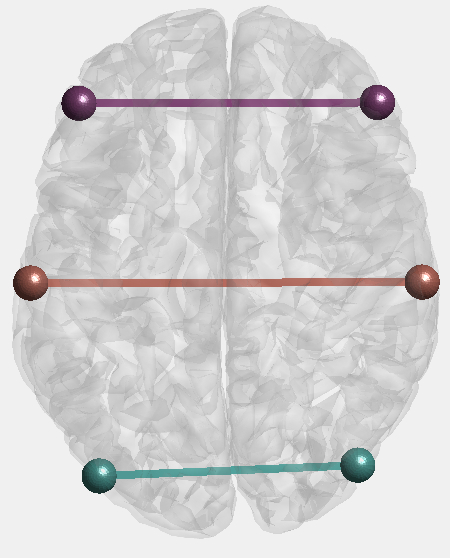
\includegraphics[angle = 90, height = 6cm]{../images/psiicos_paper/Figure2a_hr.jpg}\label{fig:2a}
        \caption{}
    \end{subfigure}
    \begin{subfigure}[t]{0.5\textwidth}
        \centering
        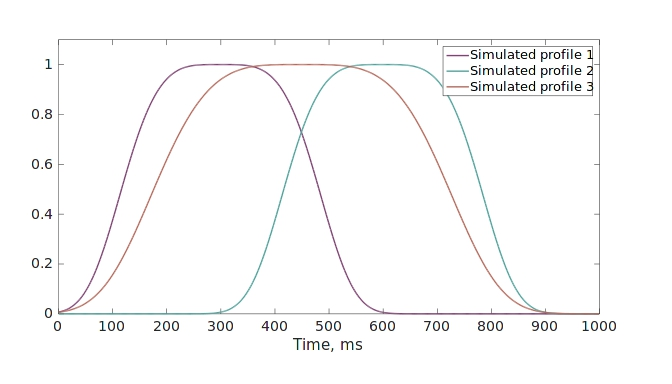
\includegraphics[width=1\textwidth]{../images/psiicos_paper/Figure2b_hr.jpg}\label{fig:2b}
        \caption{}
    \end{subfigure}
    \caption{Три симулированные пары взаимодействующих источников.}\label{02}
        (а)~--- пространственное распределение симулированных источников,
        (б)~--- временные профили активации для каждой из трех сетей.
\end{figure}


Для этих тестов мы сравнивали PSIICOS с тремя другими методами детекции
синхронных источников. Первым из этих методов был метод DICS
(см.~\ref{subsec:DICS},~\cite{Gross2001}).  При этом мы восстанавливали
элементы кросс-спектра на источниках, не нормируя их на мощность, чтобы
корректно сравнить результаты с PSIICOS.\@

Чтобы исключить влияние протечки сигнала, мы также использовали
модифицированную версию алгоритма DICS, в которой используется только мнимая
часть кросс-спектра (iDICS, см. разд.~\ref{subsec:iDICS}). Алгоритм iDICS был
вторым из набора методов, с которыми мы сравнивали PSIICOS.\@

В качестве третьего метода мы взяли алгоритм GCS~\ref{subsec:GCS}.  Как и в
оригинальной статье~\cite{Wens2015}, для построения обратного оператора мы
использовали метод MNE~\ref{subsubsec:MNE} и использовали известную матрицу
ковариации шума мозга. Алгоритму PSIICOS эта информация не нужна, и поэтому не
использовалась.

\section{Сравнение на реальных данных.}\label{sec:validation_on_real_data}

Мы применили предложенный метод для анализа реальных МЭГ-данных. Эти данные
были получены для исследования воображаемых вращений в
статье~\cite{DeLange2008}. Часть данных для одного испытуемого была выложена в
свободный доступ в ходе соревнования по анализу данных на конференции Biomag
2010.

В эксперименте испытуемый определял латеральность изображенной на экране кисти
руки нажатием на одну из двух соответствующих кнопок.  Изображения рук были
повернуты к наблюдателю на некторый угол, и для ответа испытуемый должен был
мысленно их повернуть. Авторы статьи исследовали электрическую активность коры
при осуществлении воображаемых вращений.

Данные содержали 800 эпох с рандомизированными углами поворота и
латеральностями. Эти 800 эпох были разделены на 5 блоков. Каждая эпоха включала
следующую последовательность событий: фиксационный крест (3 сек. предъявления),
изображение руки (предъявление до момента ответа испытуемого), фиксационный
крест (0.5 сек.), окрашенный в красный или зеленый цвет в зависимости от
правильности ответа испытуемого. В среднем испытуемые проводили в МЭГ-сканнере
70 минут.

В ходе эксперимента мозговая активность регистрировалась МЭГ-устройством
системы VSM/CTF Systems, включающим 151 аксиальный градиометр. Аналоговый
сигнал был отфильтрован  фильтром нижних частот с частотой среза 300 Гц и
сэмплирован на частоте 1200 Гц. После удаления артефактных сегментов для
анализа осталось 259 эпох, соответствующих изображениям левой руки. Их
длительность лежала в пределах от 1.52 сек до 2.08 сек. Мы выровняли эпохи
таким образом, чтобы начало каждой эпохи соответствовало моменту 0.5 сек до
предъявления изображения. Для анализа мы брали 1 секунду после предъявления
стимула.

Для анализа мы использовали следующие полосы частот: тета (4--8 Гц), альфа
(8--12 Гц), бета (16--24 Гц), нижняя гамма (30--60 Гц), верхняя гамма (65--85
Гц).

На первом шаге мы применяли полосовой КИХ-фильтр с нулевой фазой для отделения
целевой полосы частот. Далее мы усредняли по эпохам внешние произведения
временных рядов с примененным преобразованием в аналитический сигнал. Таким
образом мы получали временной ряд кросс-спектра в виде трехмерного массива,
который после векторизации задавался матрицей $M^2 \times T$, где $M=151$~---
количество сенсоров в установке. Далее мы применяли к временному ряду
кросс-спектра PSIICOS-проекцию с рангом $R=150$, который мы определяли исходя
из соображений, изложенных в разделе~\ref{sec:subspaces_attenuation}. Мы
проводили анализ и с другими значениями параметра $R$ в диапазоне от 100 до
250, и в этих пределах ранг проекции не оказывал значительного влияния на
решение.

Далее мы отдельно анализировали действительную и мнимую части векторизованного
временного ряда кросс-спектра. Вместо простого усреднения вдоль временной оси
для восстановления пространственной структуры мы вычисляли SVD-разложение
действительной и мнимой части спроецированного кросс-спектрального временного
ряда. Далее мы проводили поиск сетей-источников для первых двух левых
собственных векторов мнимой и действительной части на подробной сетке из 15000
узлов.

Для проверки стабильности получаемых решений мы использовали процедуру
бутстрэпа, описанную в разделе~\ref{sec:bootstrap} для $m=30$ и $B=100$ и
отрисовывали индекс воспроизводимости $\eta$.  Мы отображали полученные сети
только в рамках стабильных, воспроизводимых на бутстрэпе пучков сетей. Сети,
которые отстояли друг от друга на расстояние меньше 1см, мы рисовали одним
цветом.  Также для каждой воспроизводимой компоненты мы рисовали временной
профиль активации как правый собственный вектор временного ряда кросс-спектра.

% \section{Результаты.}\label{results}

\section{Действие проекции на компоненты кросс-спектра в пространстве источников.}\label{sec:subspaces_attenuation}

Из-за ортогональности 2-топографий действительной и мнимой частей операция
проекции никак не влияет на мнимую часть кросс-спектра. На действительную
часть, содержащую информацию о малых фазовых задержках, проекция напротив
оказывыает значительное влияние.  Удаляя часть, соответствующую протечке
сигнала, мы неизбежно удаляем и часть полезного сигнала. Качество работы
предложенного алгоритма подавления протечки сигнала в действительной части
кросс-спектра существенно зависит от следующих двух факторов:

\begin{itemize}
    \item PSIICOS-проекция должна максимально подавлять мощность компонент в
        подпространстве протечки сигнала и одновременно с этим минимально
        изменять мощность истинной действительной части когеренции.
    \item Как и для всех алгоритмов решения обратной задачи PSIICOS-проекция
        существенно зависит от точности прямой модели. Неизбежная погрешность
        при ее построении~\cite{Mosher1999} оказывает соответствующее влияние
        на качество решений предложенного метода. Вместе с тем, ошибки прямой
        модели в разумных пределах должны вызывать лишь незначительное
        ухудшение качества решения.
\end{itemize}

Степень выполнения этих условий зависит от феноменологических характеристик
массива сенсоров, а также от магнитных топографий имеющихся мозговых
источников. В этом разделе мы опишем результаты численного моделирования,
направленного на изучение этой проблемы.

Подавление мощности в подпространстве действительной части кросс-спектра
очевидным образом проявляется наиболее сильно для источников с кореллированными
топографиями.  Для исследования зависимости подавления от коэффициента
корреляции между топографиями взаимодействующих источников для каждой пары
индексов $i, j$ мы вычисляли нормы до и после проекции для 2-топографий вида
$\vec{g}_i \otimes \vec{g}_i + \vec{g}_j \otimes \vec{g}_j$,
$\vec{g}_j\otimes\vec{g}_i + \vec{g}_i\otimes\vec{g}_j$ а также
$\vec{g}_j\otimes\vec{g}_i - \vec{g}_i\otimes\vec{g}_j$, соответствующие
подпространствам $S^{SL}, S^{\Im}, S^{\Re}$. Результаты представлены на графике~\ref{fig:02}.

\begin{figure}[!ht]
 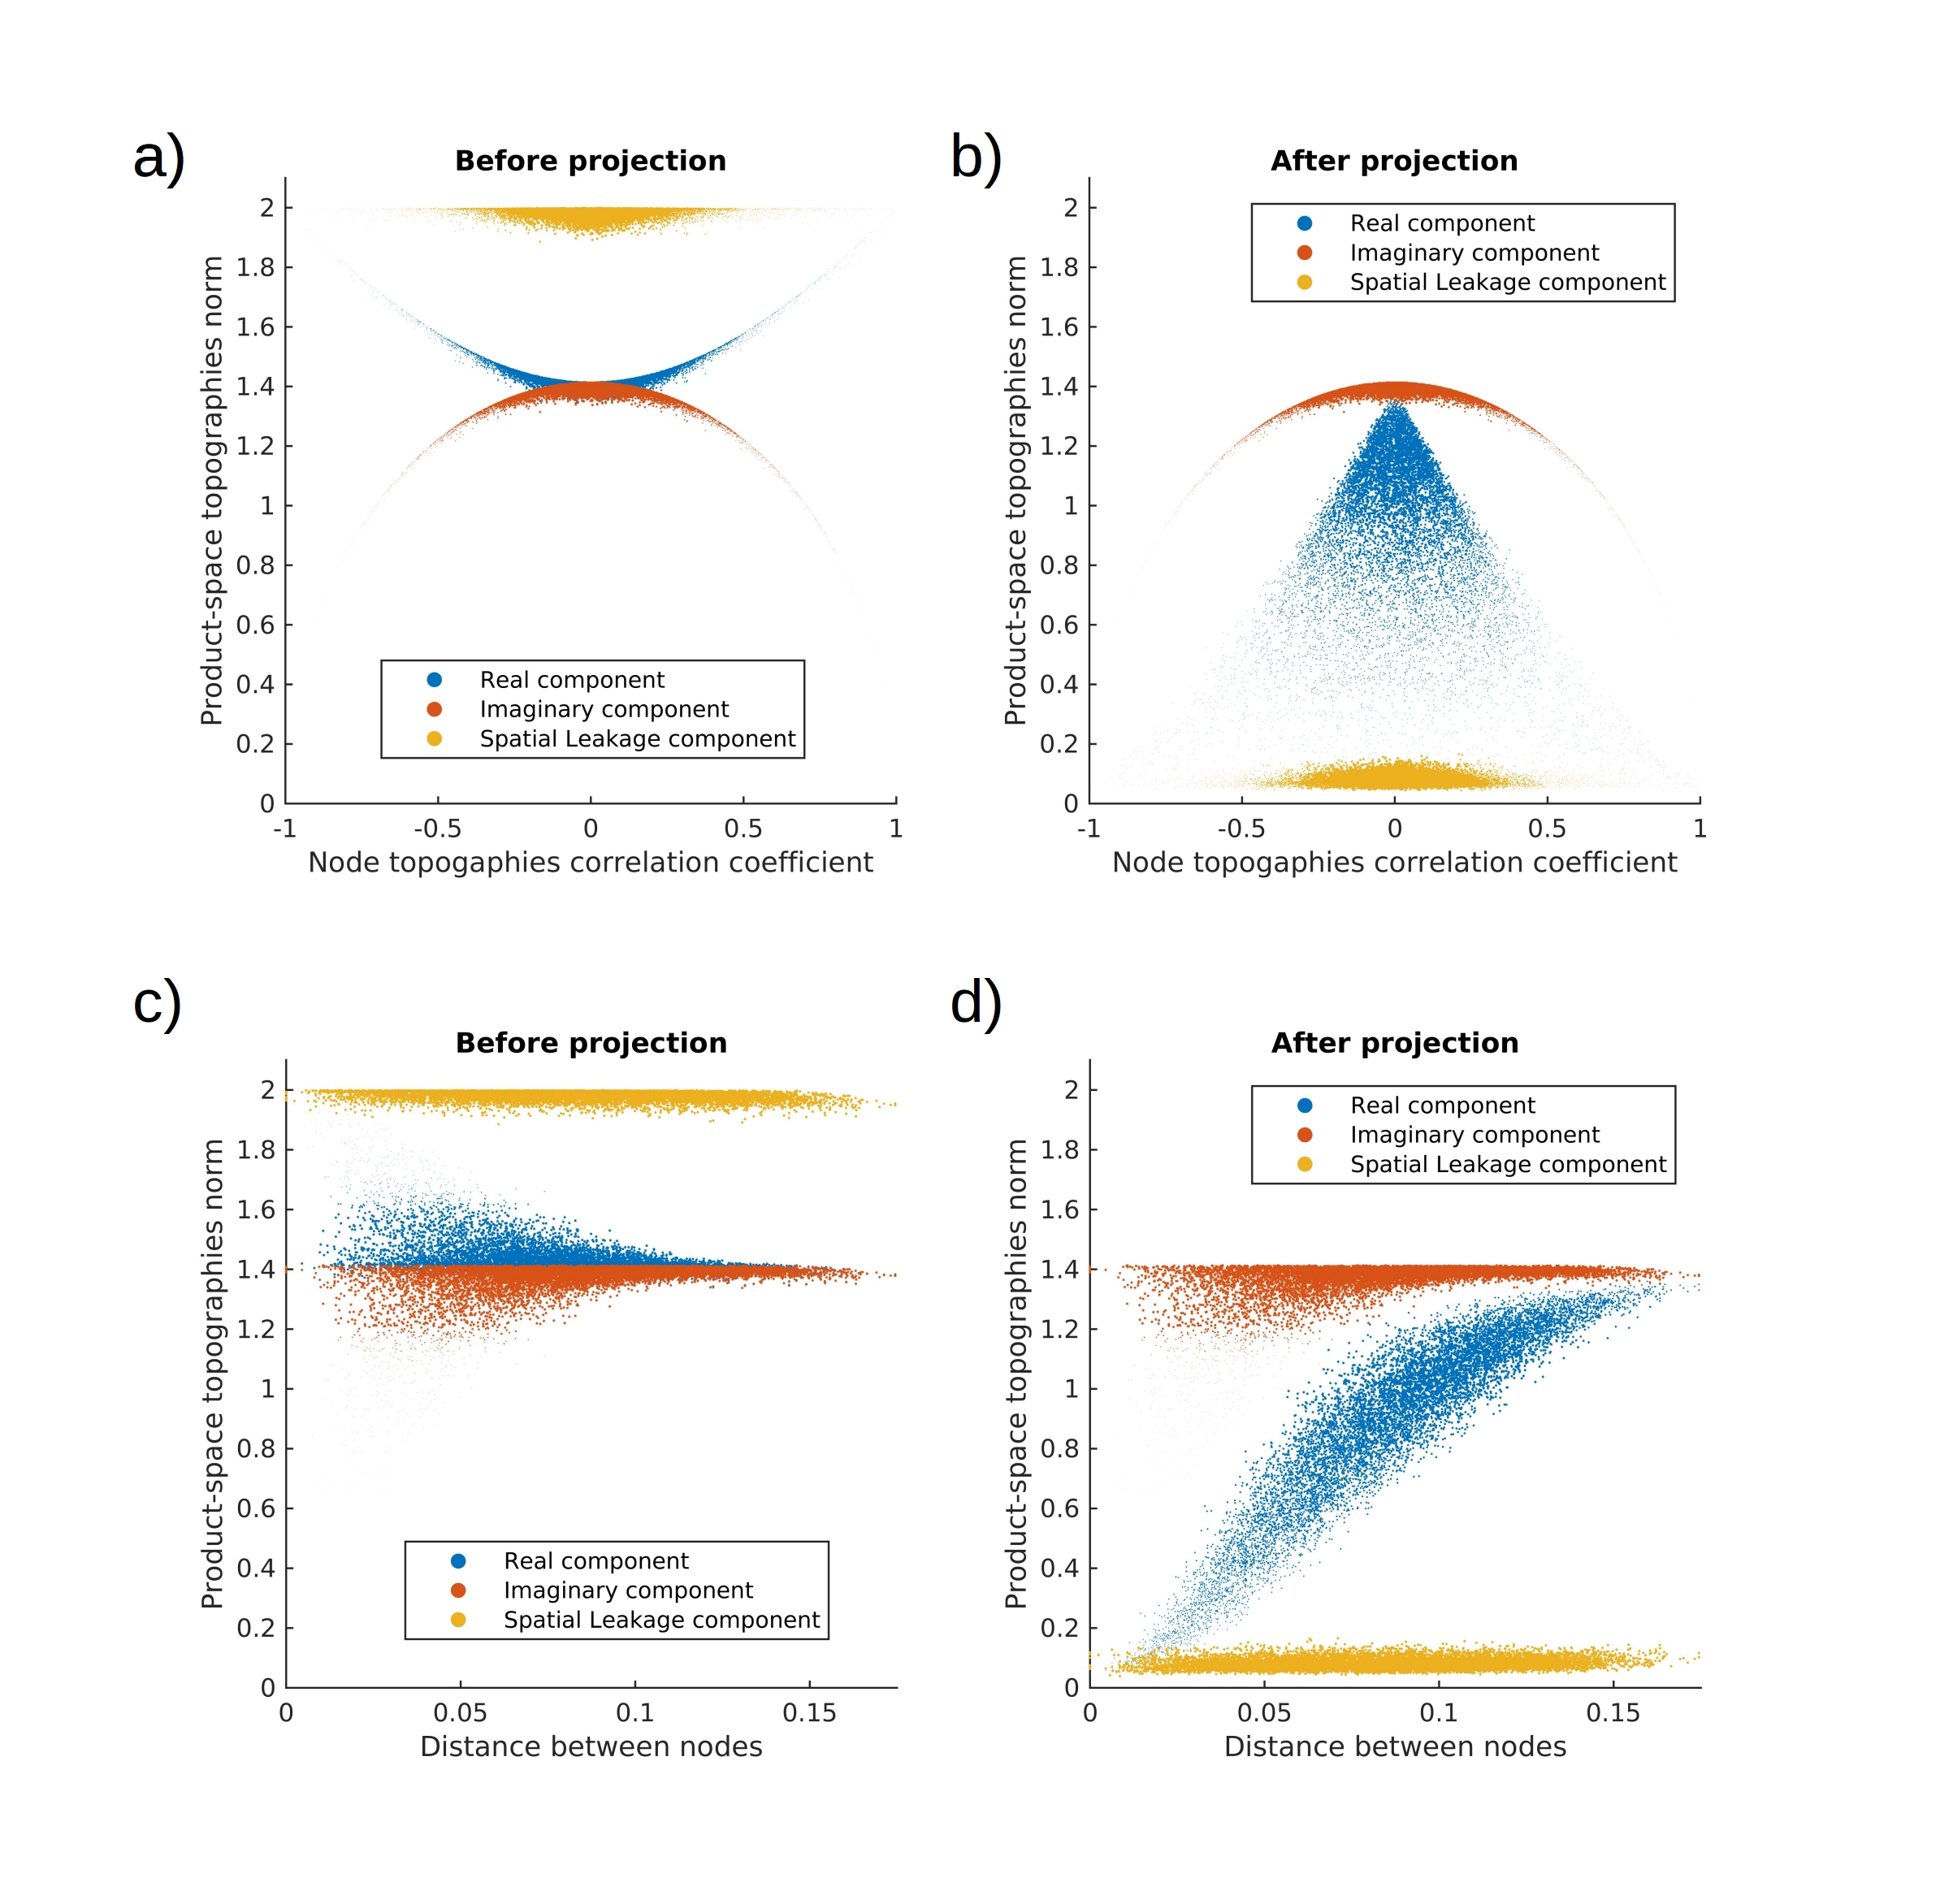
\includegraphics[width=1\textwidth]{../images/psiicos_paper/Figure3abcd_hr}
 \caption{Нормы 2-топографий для трех подпространств кросс-спектра до и после проекци
     в зависимости от коэффициента корреляции топографий взаимодействующих
     узлов на коре (графики (a) и (b)), а также от расстояния между
     этими узлами (графики (c) и (d)).}\label{fig:02} % Figure 3 in the text
     До проекции (графики (a), (c)) в кросс-спектр на уровне сенсоров наибольший вклад дает мощностная
     компонента (обозначена желтым цветом). После проекции (графики (b), (d))
     вклад мощностной компоненты уменьшается в среднем в 25 раз. Вместе с
     тем наблюдается неизбежное, но значительно меньшее ослабление
     2-топографий действительной части, соответствующих истинной коннективности.
     В среднем они ослабляются в 1.6 раз.
\end{figure}

Для каждой сети с узлами в точках $i$ и $j$ на коре соответствует три точки
разных цветов на графике: красная, синяя и желтая. Градации синего цвета мы
использовали для кодировки информации о величине нормы 2-топографии
действительной части $\vec{g}_j\otimes\vec{g}_i + \vec{g}_i\otimes\vec{g}_j$.
Градации красного цвета использовались для 2-топографий мнимой части, и
желтого~--- для топографий протечки сигнала.  Положение каждой цветной точки
вдоль оси $x$ для подграфиков (a), (b) определялось величной коэффициента
корреляции топографий $\vec{g}_i$ и $\vec{g}_j$.  Кроме того, мы отобразили те
же самые данные на втором графике, где вместо корреляции по оси $x$
использовалось расстояние между узлами сети $i, j$. Насыщенность цвета точек
отражает плотность точек в соответствующей области графика.

\section{Влияние неточностей прямой модели на качество решений}\label{sec:forward_model_errors_effect}

В этом разделе мы исследовали влияние неточностей в прямой модели на качество
работы предложенного алгоритма. Оказвается, что хотя неточности прямой модели и
вызывают ухудшение решений метода, для типичных в прямых моделях для МЭГ
уровней шума порядка 10\% (\cite{Mosher1999}), проекция подавляет мощность в
подпространстве протечки сигнала почти так же хорошо и лишь на 20\% сильнее
подавляет подпространство действительной части.

\section{Сравнительный анализ.}

 В этом разделе мы описали результаты сравнения предложенного метода PSIICOS
 с тремя другими методами для обнаружения синхронных источников: DICS, iDICS и GCS.\@

\subsection{Анализ ROC-кривых методом Монте-Карло.}
Чтобы количественно охарактеризовать качество детекции сетей методом PSIICOS для различных
пространственных конфигураций сетей, мы провели анализ методом Монте-Карло в соответствии
с процедурой, описанной в разделе~\ref{sec:monte_carlo_simulation}.

На графике~\ref{fig:07} видно, что для каждого из условий симуляции качество решений
алгоритма PSIICOS стабильно превосходит другие методы и позволяет получать решения хорошего
качества независимо от величины фазовой задержки.

По графику ROC-кривой для средней разницы фаз $\delta\phi=\pi/2 - \pi/20$ видно, что
показатели iDICS сравнимы с показателями PSIICOS.\@Однако для $\delta\phi = \pi/20$ iDICS
не способен адекватно распознавать сети в силу значительного снижения ОСШ, вызванного
тем, что сети с близкой к нулю фазовой задержкой дают очень маленький вклад во
мнимую часть кросс-спектра.

Метод MNE GCS ведет себя лучше, чем DICS для высоких значений ОСШ. Для низкого ОСШ
оба метода показывают плохие результаты. В то же время метод PSIICOS демонстрирует
адекватное качество решения для обоих значений ОСШ.

В случае низкого ОСШ большая разница в качестве решения PSIICOS между двумя
значениями фазовых задержек вероятно объясняется наличием в итерациях
Монте-Карло сетей с пространственно близкими узлами. Это приводит к тому, что
действительная часть членов, соответствующих истинному взаимодействию,
значительно искажается проекцией. Вместе с тем, остальные методы при таких
условиях для практически перестают работать в случае близких к нулю фазовых задержек.

\subsection{Обнаружение нескольких одновременно активных сетей.}

В этом разделе мы описали результаты, полученные при симулировании трех сетей с
перекрывающейся во времени активностью (см.~\ref{sec:monte_carlo_simulation}).
Для этого анализа мы фильтровали симуляционные данные в полосе 8--12 Гц и
вычисляли временной ряд кросс-спектра для каждого временного среза усреднением
по эпохам внешних произведений аналитических сигналов.

На графике~\ref{fig:05} изображена пространственная структура решения для
симуляционных данных в пространстве источников. На графике отображены 0.1\% сетей
с максимальными значениями статистики, оцененной методом PSIICOS и другими тремя
алгоритмами. Как видно из графика, алгоритм PSIICOS сохраняет адекватное качество решения
для всего спектра тестируемых условий.

\begin{figure}[!ht]
 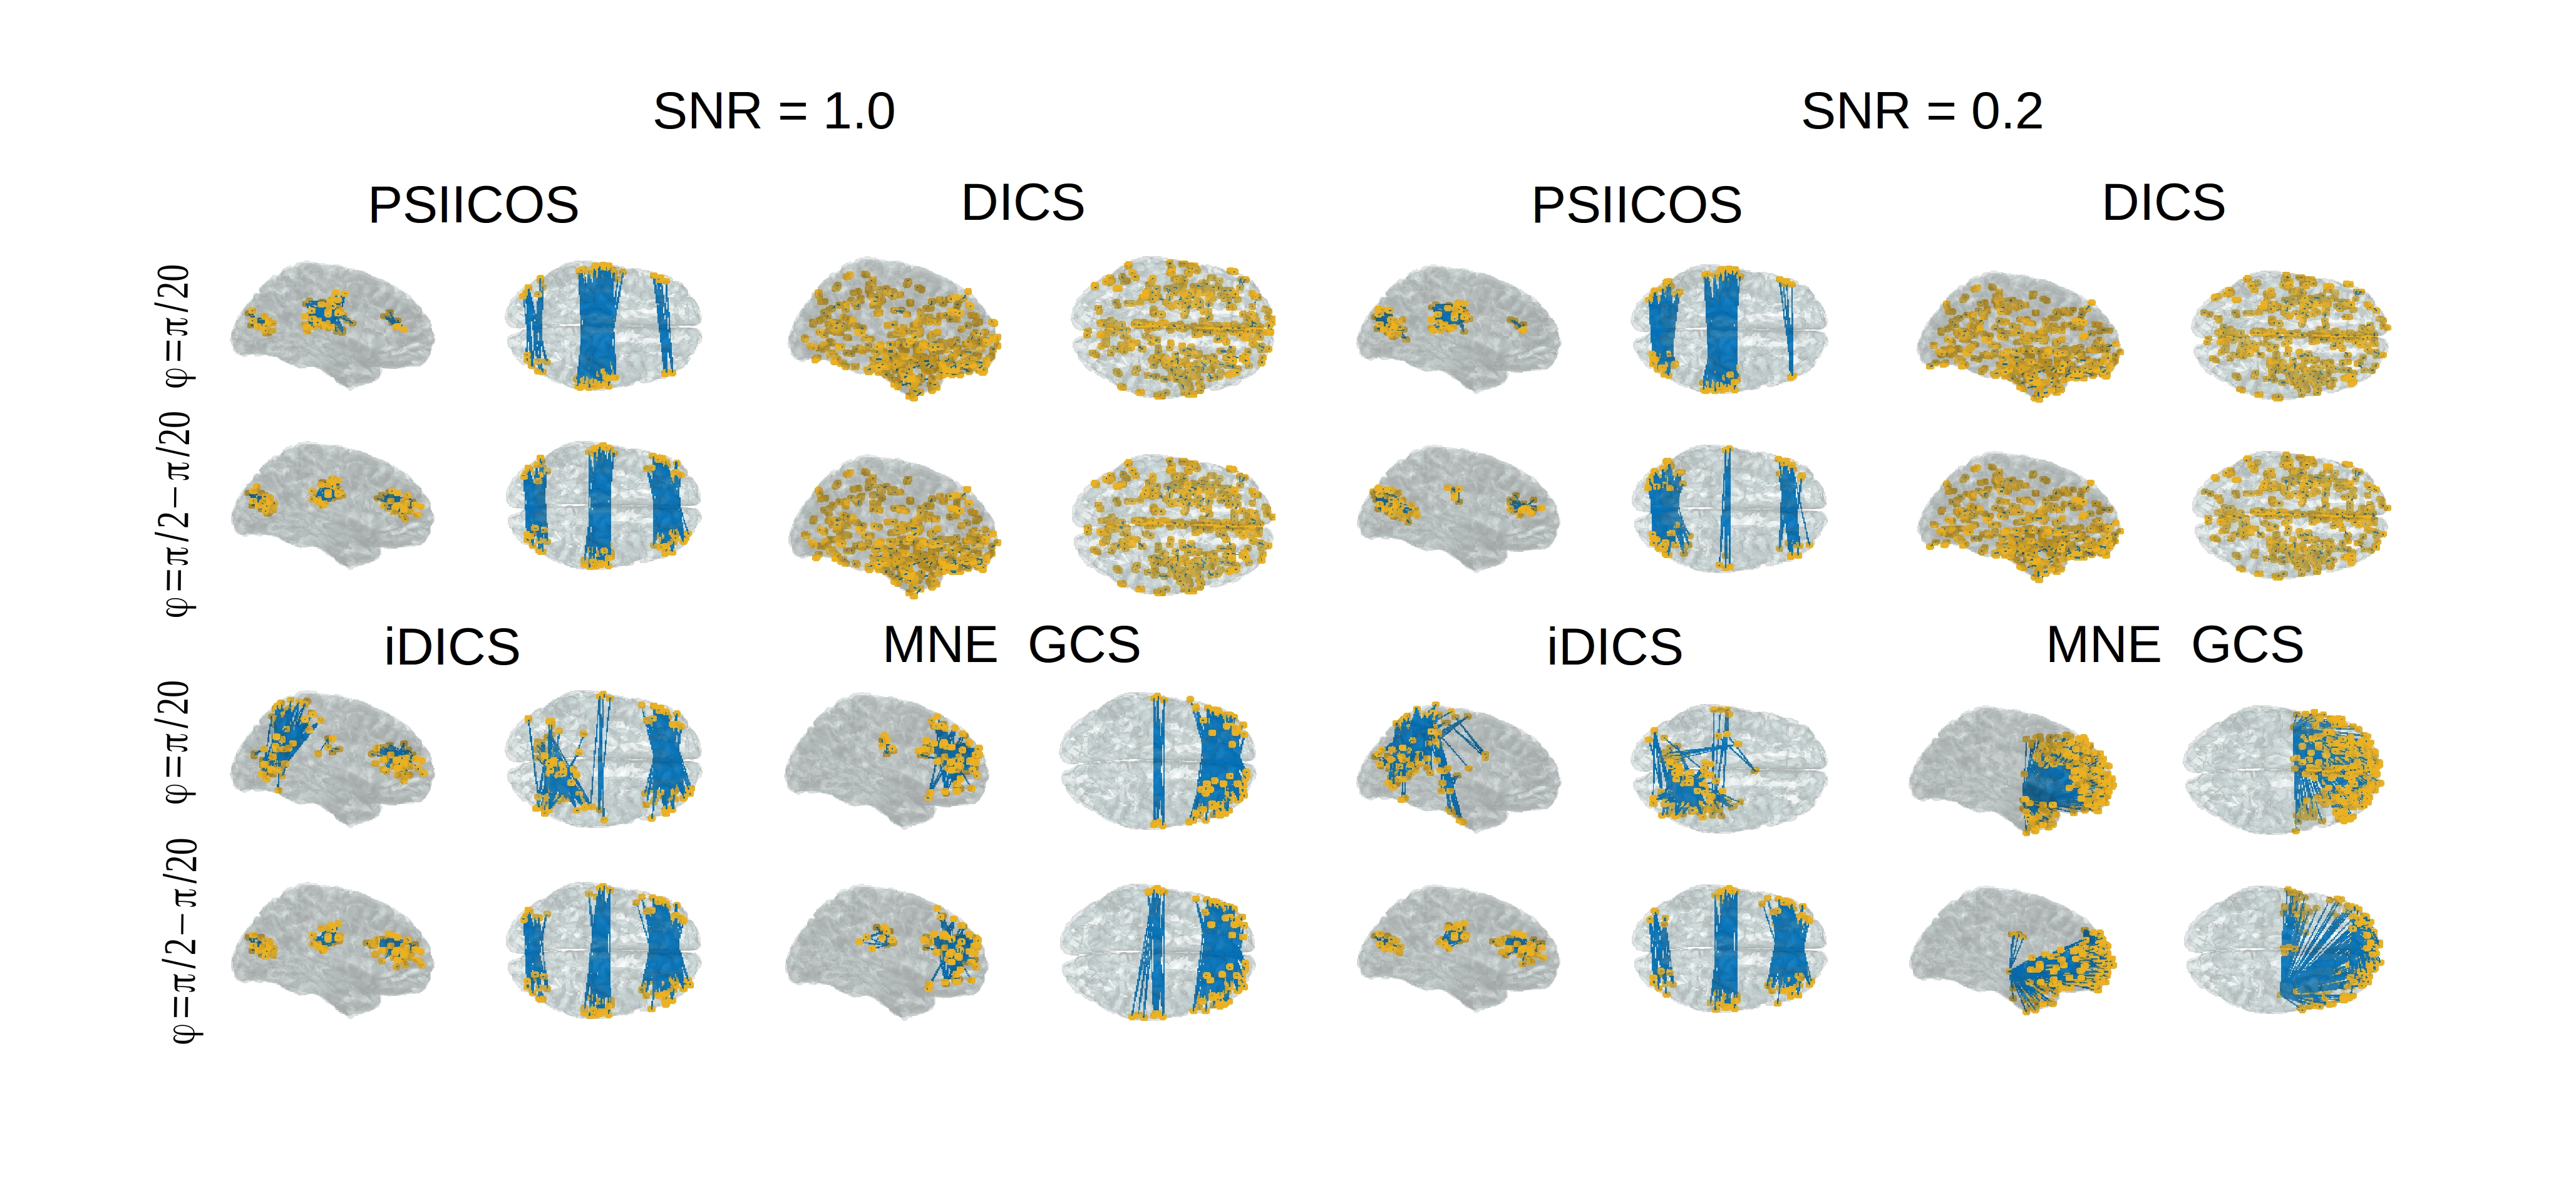
\includegraphics[width=1\textwidth]{../images/psiicos_paper/Figure5_hr.jpg}
 \caption{Пространственное распределение сетевых источников для симуляционных данных.}\label{fig:05} %Figure 5
     На графике изображены 0.1\% сетей с наибольшим значением
     статистики. Из графиков видно, что только алгоритм PSIICOS сохраняет
     качество решения для всего диапазона изучаемых значений.
     Метод iDICS ведет себя практически также хорошо, как и PSIICOS,
     для фазовых сдвигов, близких к $\pi/2$, что согласуется с нашими предыдущими
     результатами. Метод MNE GCS для высоких значений ОСШ достаточно надежно определяет
     две фронтальные сети для каждого значения фазового сдвига, но полностью перестает
     работать для низких значений ОСШ и близких к нулю фазовых задержек. Для задержек,
     близких к $\pi/2$, при низком ОСШ этот метод находит только среднюю сеть
     (для нее индивидуальное ОСШ выше всего) а также порождает большое количество
     ложноположительных срабатываний.
\end{figure}%

Как и для симуляций в разделе~\ref{sec:monte_carlo_simulation}, метод iDICS показывает себя
практически так же хорошо, как и PSIICOS для значений фазовой задержки, близких к $\pi/2$.
Метод MNE GCS для случая высокого ОСШ достаточно надежно определяет две фронтальные сети для
обоих значений фазовой задержки, но полностью перестает работать для низкого ОСШ и
околонулевой разности фаз. Для случая фазовой задержки, близкой к $\pi/2$, и низкого ОСШ
MNE GCS обнаруживает только среднюю сеть (сеть с наибольшим индивидуальным ОСШ) и
порождает большое количество ложно-положительных сетей.

Умножая временной ряд кросс-спектра на сенсорах на среднюю топографию
полученных кластеров, можем восстановить временную активность сетей.
На~\ref{fig:06} изображены временные окна, в течение которых каждая пара
взаимодействующих источников была активна.  Для построения этого графика мы
испольльзовали спроецированный от протечки сигнала временной ряд кросс-спектра,
к которому мы применяли наиболее простую процедуру оценки источников ---
фильтр, максимизирующий SNR в заданной точке~\ref{subsubsec:max_snr_filter}, с
той разницей, что здесь все операции проводились в пространстве 2-топографий с
размерностью $M^2$.

\begin{figure}[!ht]
    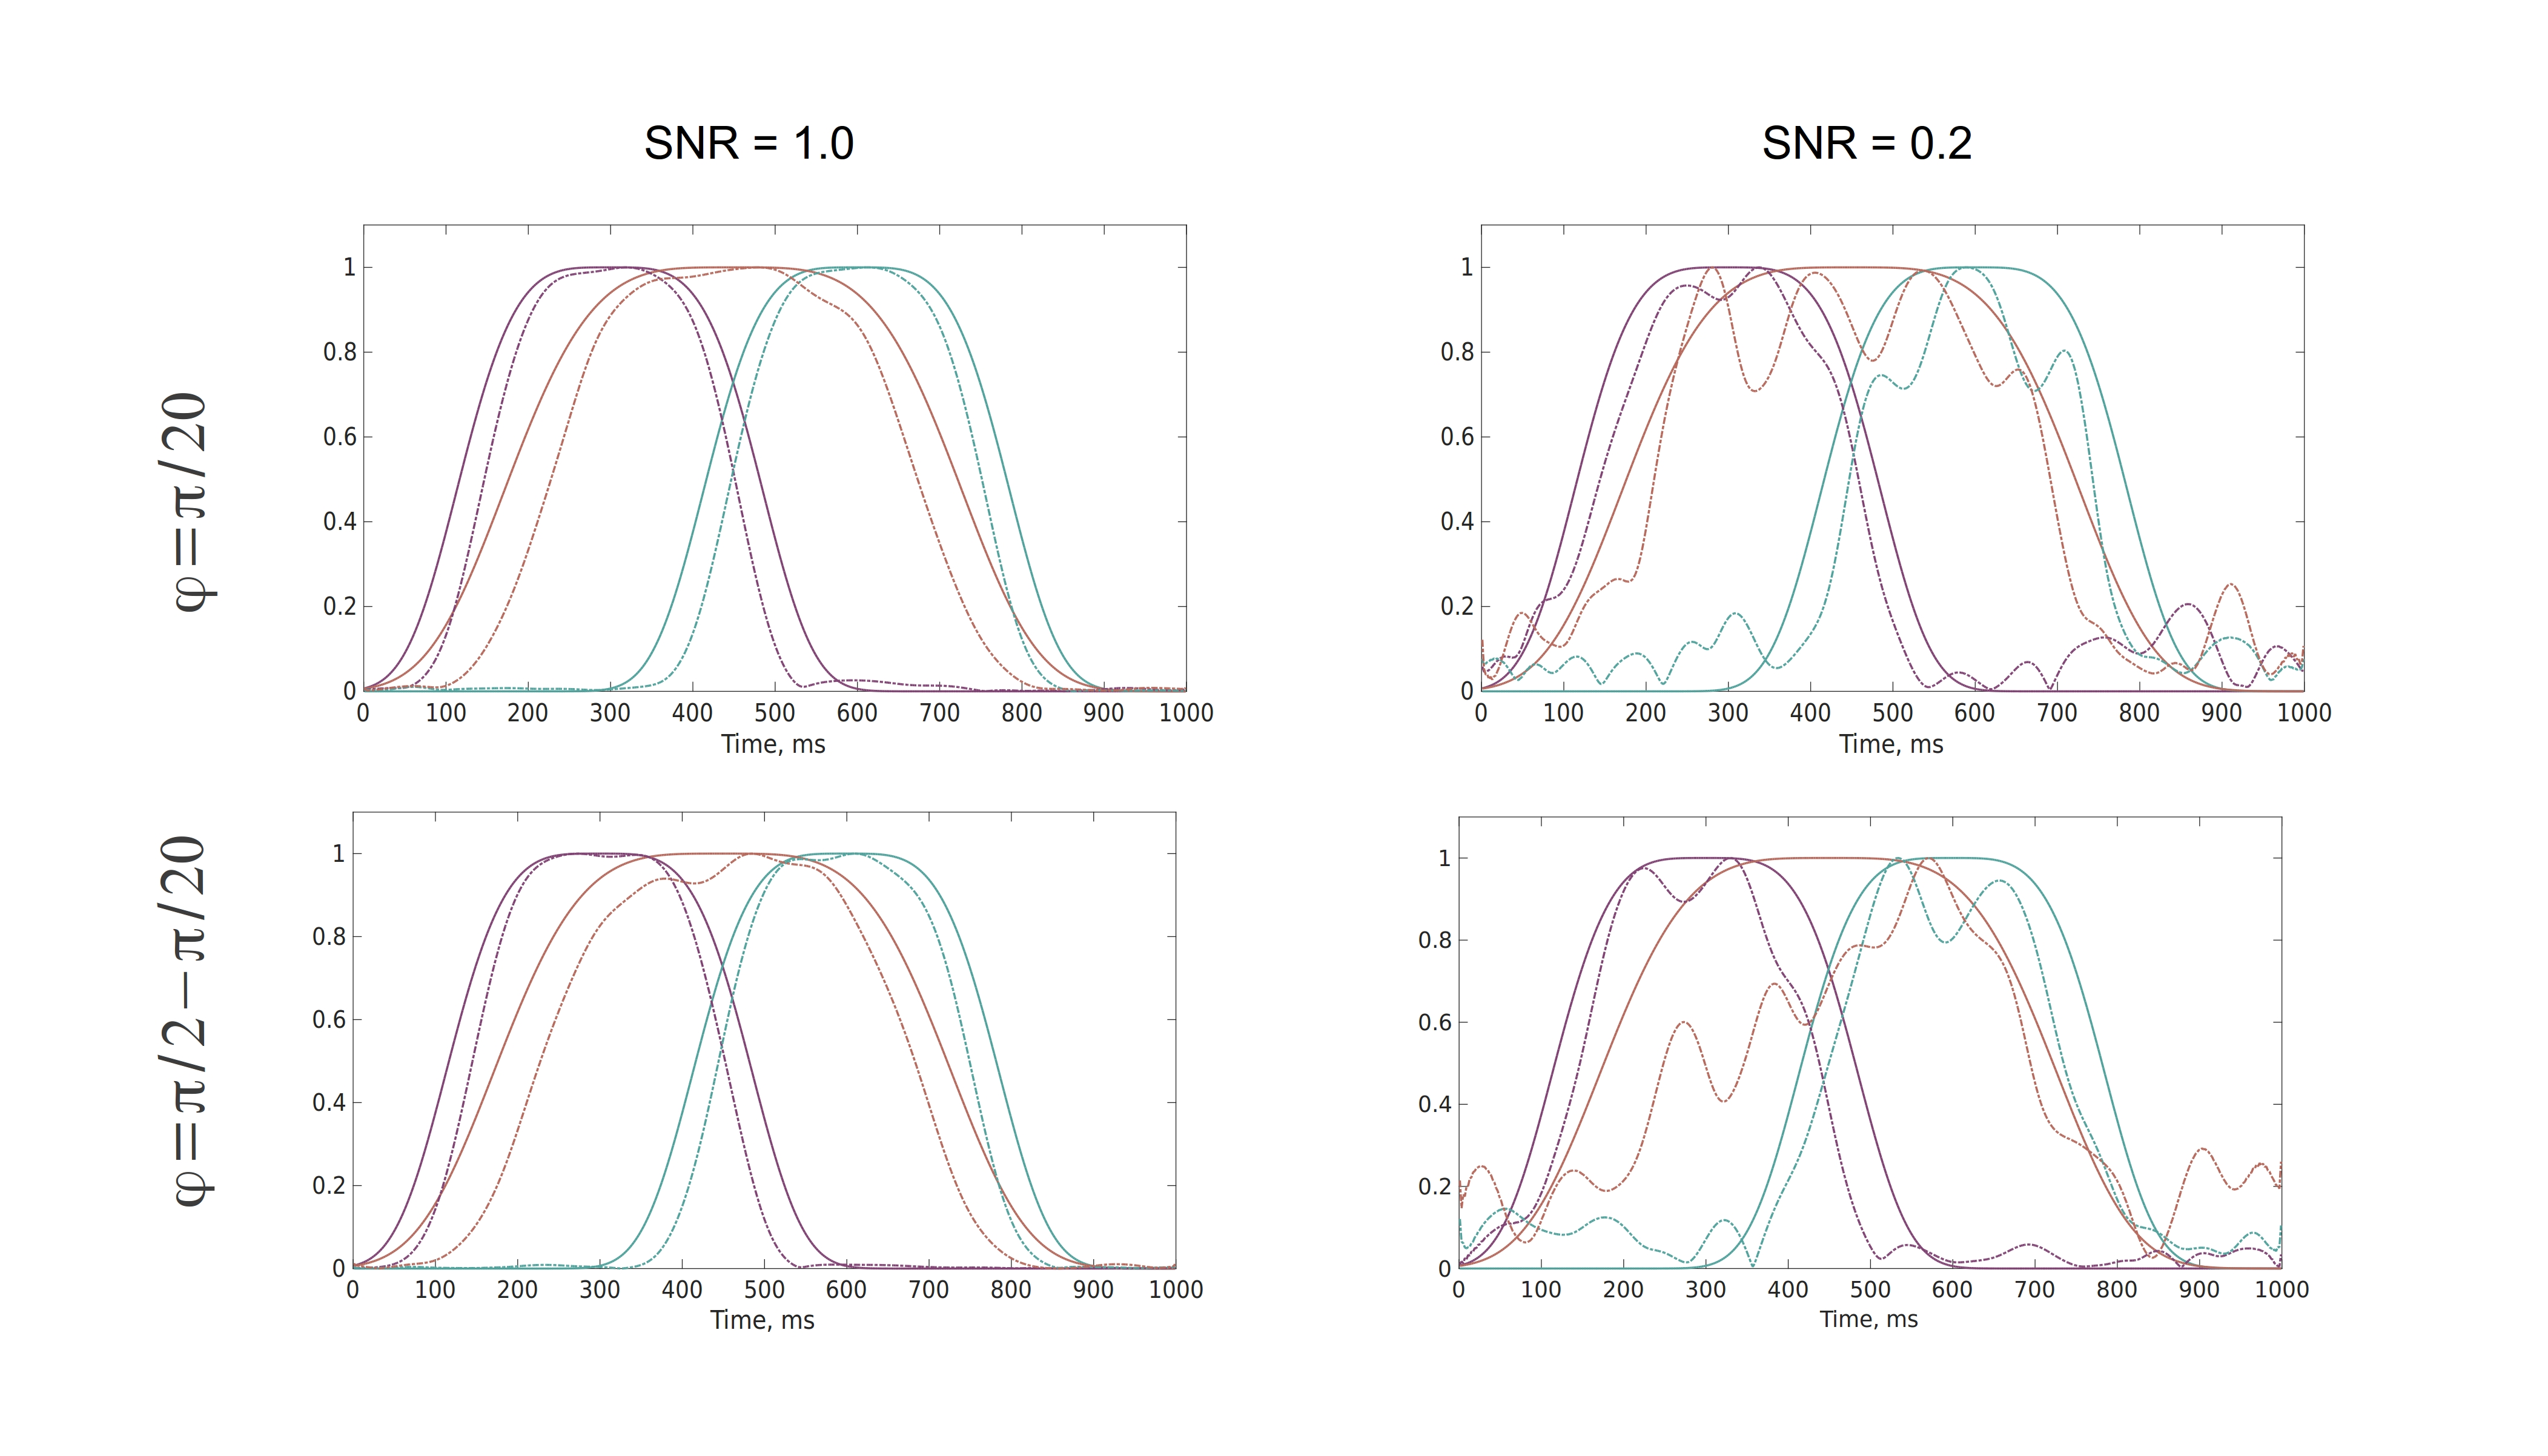
\includegraphics[width=1\textwidth]{../images/psiicos_paper/Figure6_hr.jpg}
    \caption{Временные профили активации симулированных сетей, восстанновленные при помощи PSIICOS, для двух
        значений фазового сдвига и двух значений ОСШ.}\label{fig:06} %Figure 6
        Непрерывные линии отображают истинные симулированные профили, а
        пунктир~--- восстановленные алгоритмом PSIICOS.\@
\end{figure}%

Далее, для системного сравнения четырех рассматриваемых методов на графике~\ref{fig:07}
мы модифицированные кривые Precision-Recall, на которых размером маркера мы отобразили
количество истинных сетей, обнаруженных алгоритмом. На левой части рисунка изображен
полный график Precision-Recall; на панелях (b) и (d) показаны данные в диапазоне 0--0.15.

\begin{figure}[!ht]
 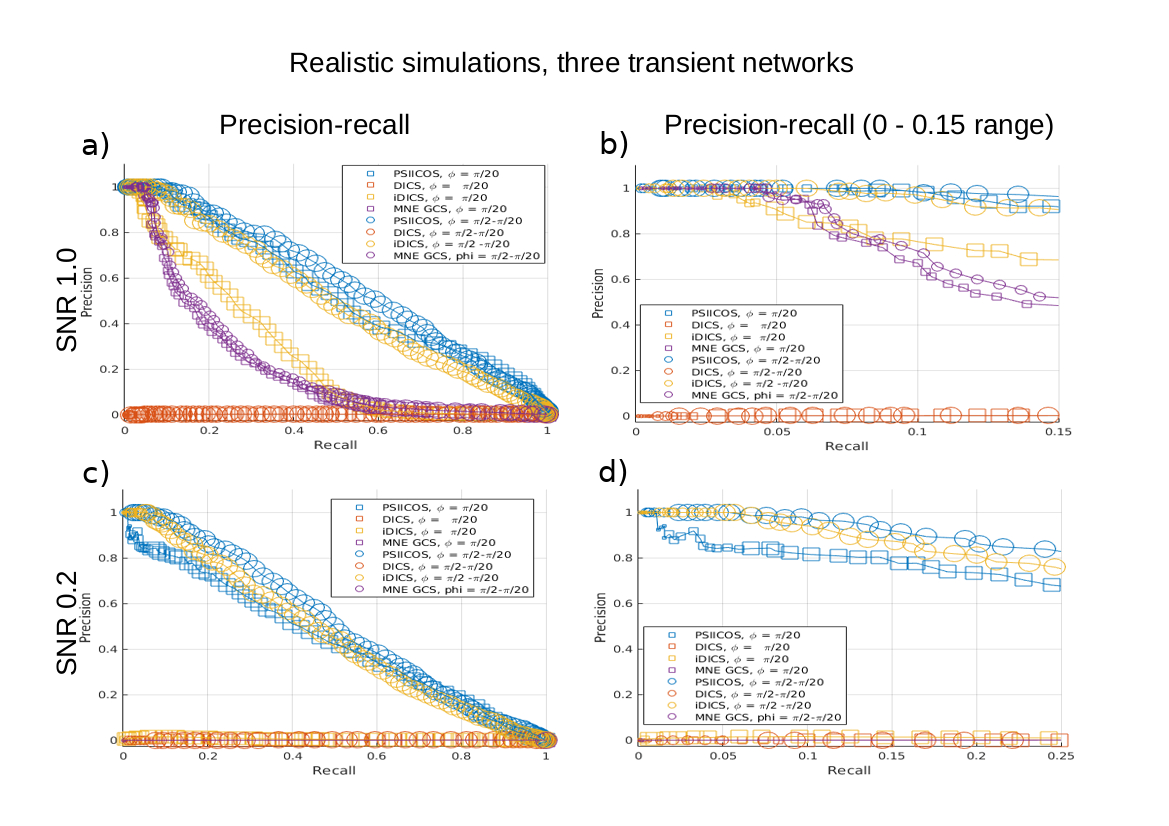
\includegraphics[width=\textwidth]{../images/psiicos_paper/Figure7_hr.jpg}
 \caption{Сравнение PSIICOS с остальными методами в задаче обнаружения трёх
 одновременно активных сетей.}\label{fig:07} %Figure 7
 На рисунках (a), (c) изображены кривые Precision-Recall для всего диапазона
 возможных значений; на рисунках (b), (d) изображены те же кривые, но для
 диапазона значений 0--0.15.
\end{figure}%

Структура этих графиков подтверждает выводы, основанные на визуальном анализе
пространственного распределения обнаруженных сетей (см. рис.~\ref{fig:05}).

Использованные до сих пор метрики оценивают качество решения независимо от порога,
что не годится для оценки качества работы алгоритма на реальных данных.
Для применения к реальным данным мы предлагаем использовать процедуру бутстрэпа,
описанную в разделе~\ref{sec:bootstrap}, чтобы оценить стабильность
получаемых решений и использовать ее в качестве метрики качества.
График~\ref{fig:08} иллюстрирует результаты процедуры
бутстрэпа в применении к реалистичным симуляционным данным.

\begin{figure}[!ht]
 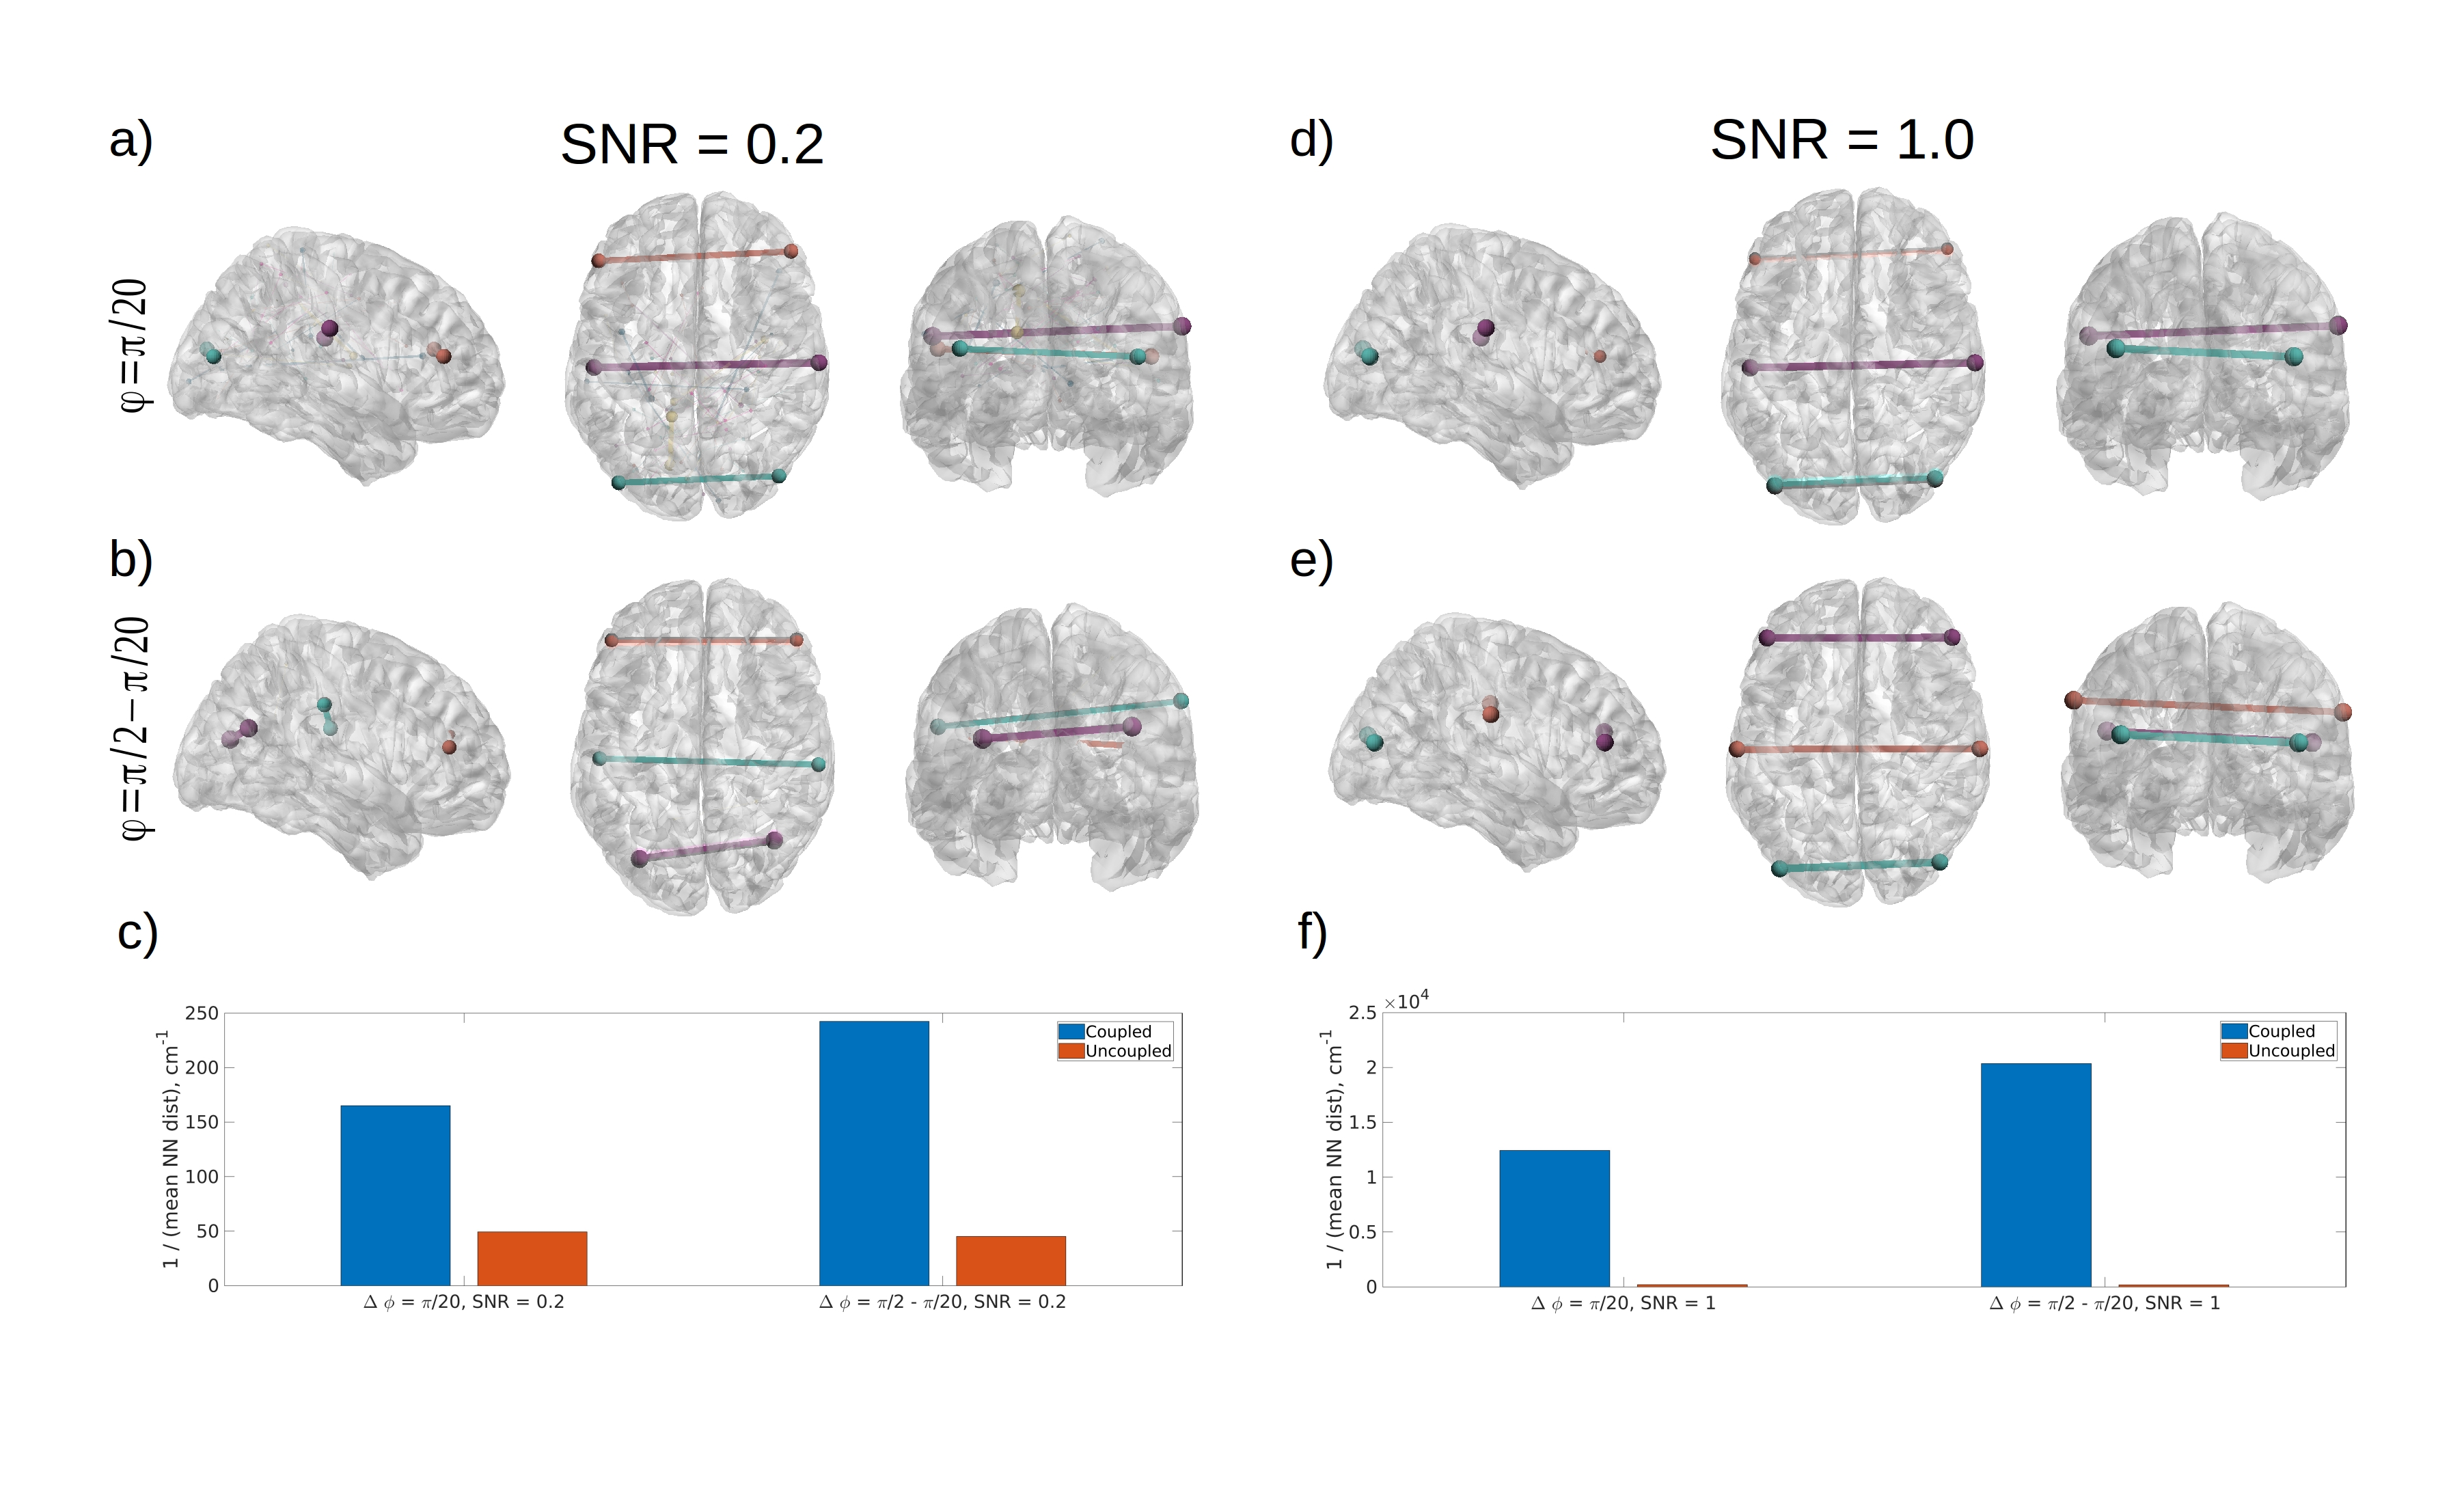
\includegraphics[width=\textwidth]{../images/psiicos_paper/Figure8_hr.jpg}
 \caption{Исследование стабильности метода PSIICOS при помощи процедуры бутстрэпа для
 двух значений фазового сдвига и двух ОСШ.}\label{fig:08}
 (a), (b), (d), (f)~--- стабильные сети отображены в виде отрезков, концы которых
 соответствуют взаимодействующим областям коры. Насыщенность цвета отрезка
 и его концов прямо пропорциональна коэффициенту воспроизводимости $\eta$,
 оцененному при помощи процедуры бутстрэпа. Отрезки, концы которых
 оказывались ближе 1 см друг к другу, мы рисовали одним цветом.
 На графиках (c) и (d) изображен индекс воспроизводимости $\eta$ для
 двух средних фазовых сдвигов, полученных в результате описанной процедуры
 бутстрэпа для двух различных значений ОСШ (ОСШ=0.2 и ОСШ=1 соответственно).
\end{figure}% Figure 8


Наши симуляции показывают, что предложенный подход позволяет достичь лучшего
качества решений при поиске взаимодействующих источников как при околонулевых,
так и при близких к $\pi/2$ фазовых сдвигах. Более того, алгоритм PSIICOS
позволяет обнаруживать сети для всего спектра возможных фазовых задержек. Чтобы
дополнительно проиллюстровать это качество, мы применили предложенный метод к
симуляционным данным с тремя сетями на равномерной сетке фазовых задержек в
диапазоне от 0 до $\pi/2$. Этот анализ мы провели для двух значений ОСШ и
сравнили три различных подхода: использование только мнимой части (iDICS),
использование только спроецированной действительной части и использование
полной кросс-спектральной матрицы (PSIICOS). На графике~\ref{fig:09}
изображена метрика качества решения в каждом из случаев для различных фазовых
сдвигов.  В качестве метрики мы использовали площадь под кривой
Precision-Recall. Для значений фазы, близких к $\pi/2$, информация о взаимодействующих
источниках содержится в основном во мнимой части кросс-спектра, что легко
заметить из графика~\ref{fig:09}, где использование только мнимой части позволяет достичь
высокого качества решения для близких к $\pi/2$ фазовых сдвигов. Для реалистичного
значения ОСШ=0.1 качество решения резко ухудшается как только значение фазового сдвига
покидает окрестность точки $\pi/2$.

\begin{figure}[!ht]
 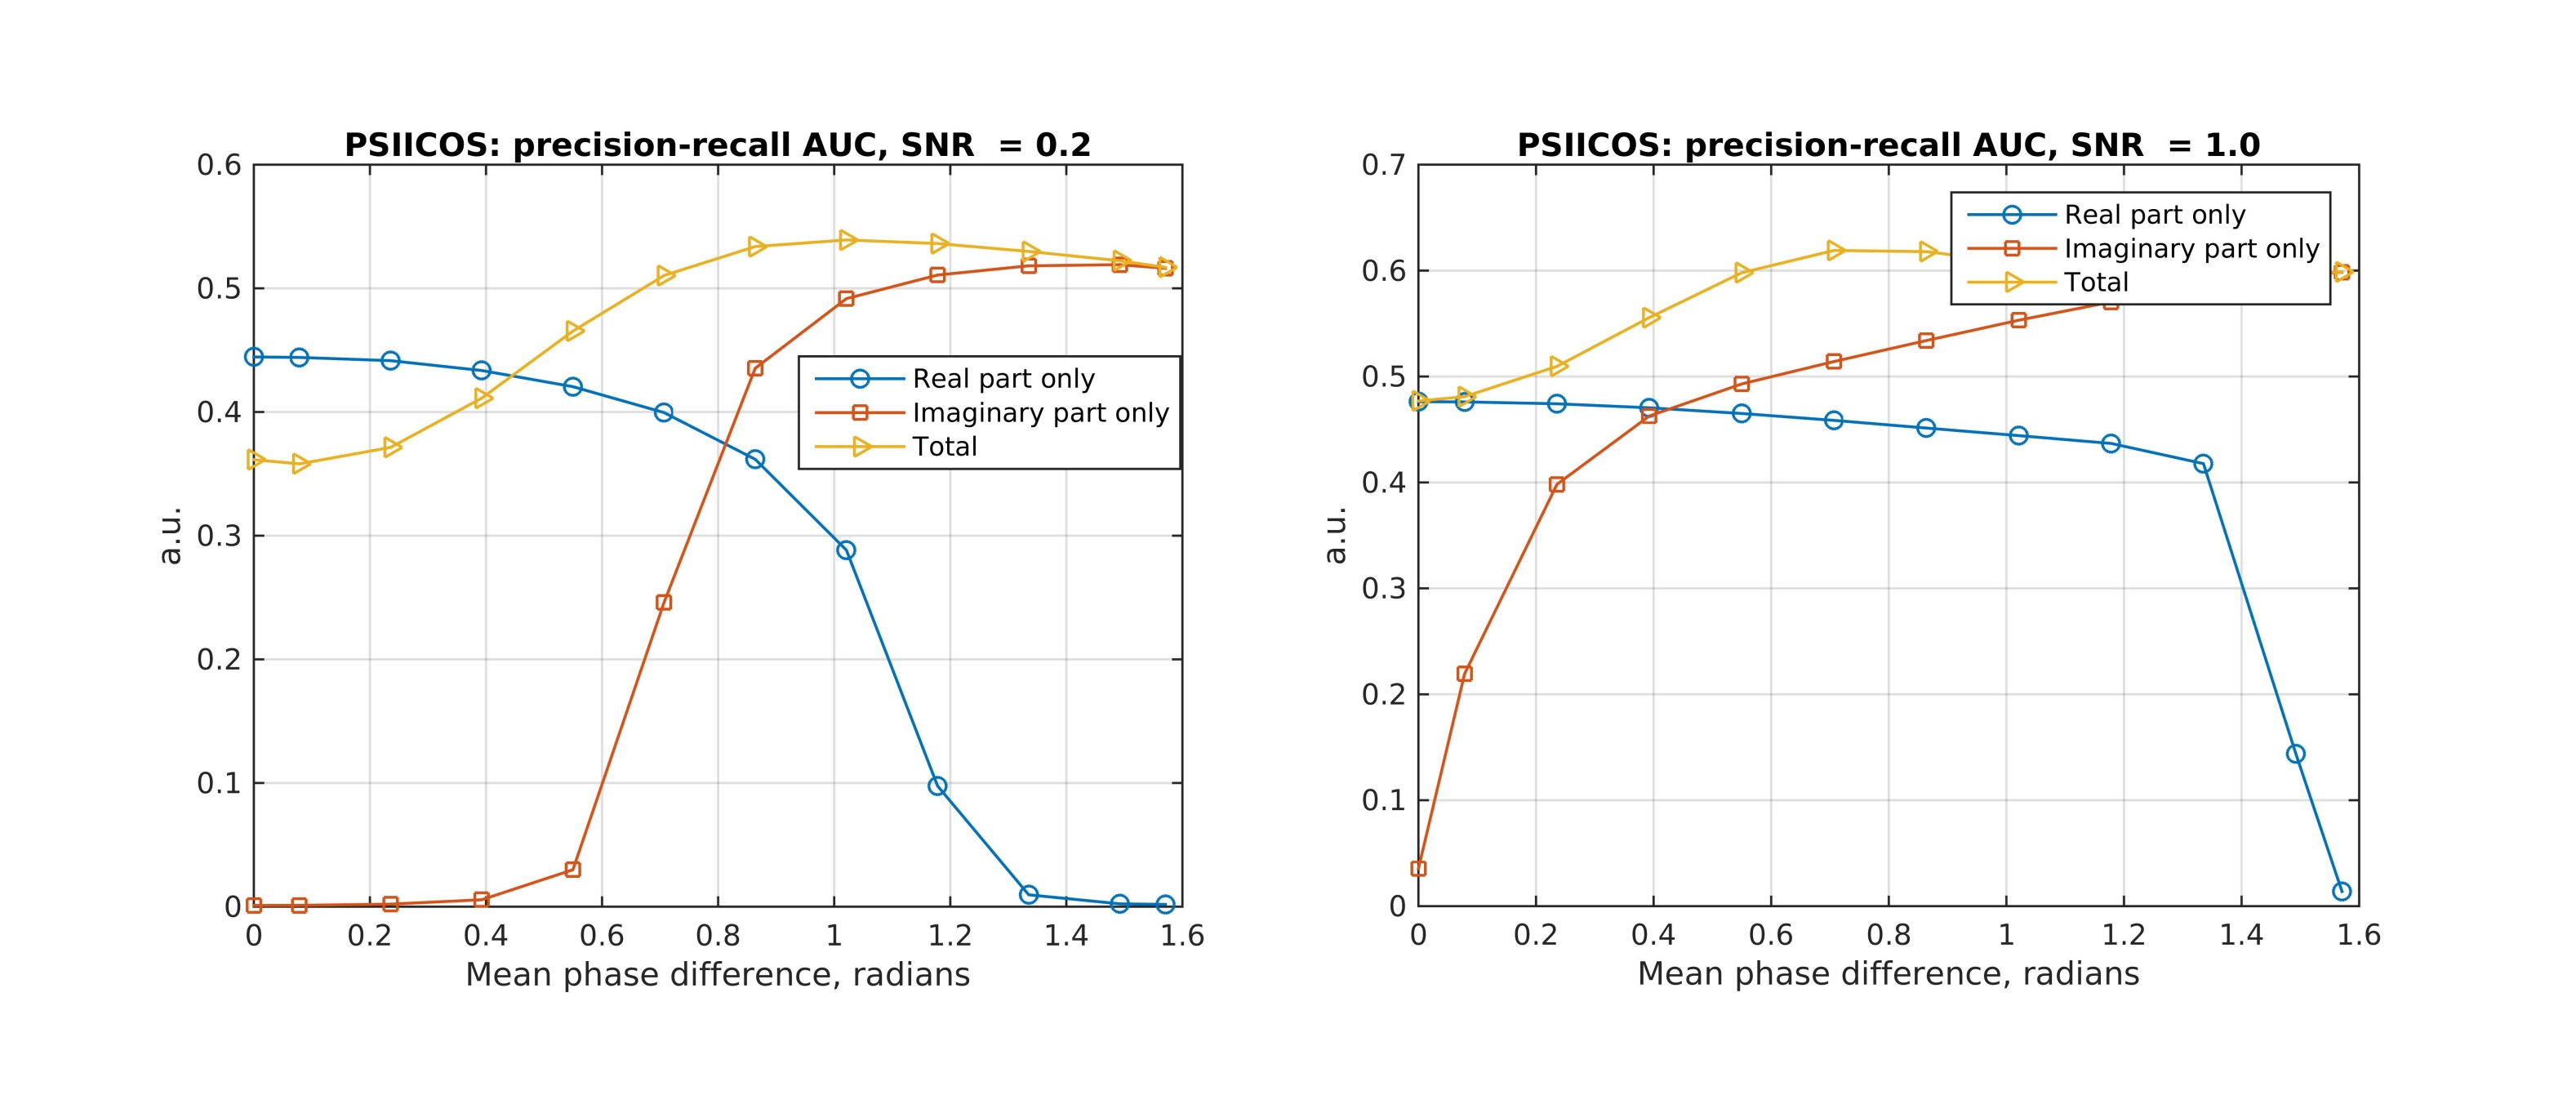
\includegraphics[width=1\textwidth]{../images/psiicos_paper/Figure9_hr.jpg}
 \caption{Качество решений алгоритма PSIICOS как функция средней фазовой задержки}\label{fig:09}
     (a)~--- для низкого значения ОСШ и (b)~--- для высокого.
     Для близких к $\pi/2$ средних значений фазового сдвига информация
     о взаимодействии источников содержится в основном во мнимой части кросс-спектра.
     Поэтому использование только мнимой части (что эквивалентно iDICS) позволяет
     достигать высокого качества решения; качество решения при этом затухает
     с уменьшением фазового сдвига. С другой стороны, для близких к нулю
     значений фазовой задержки информация о взаимодействии содержится в основном
     в действительной части кросс-спектра. Действительная часть загрязнена
     протечкой сигнала, которая может быть удалена при помощи PSIICOS-проекции.
     После этого очищенная действительная часть используется для обнаружения
     сетей с близкими к нулю фазовыми задержками (синие кривые). Одновременное
     использование действительной и мнимой компоненты позволяет добиться равномерного
     качества решений по всему диапазону средних фазовых сдвигов (оранжевая кривая).
\end{figure}% Figure 9

С другой стороны, для близких к нулю сдвигов информация о коннективности содержится
в основном в действительной части. Действительная часть загрязнена протечкой сигнала, которую
мы эффективно удаляем PSIICOS-проекцией. Далее спроецированная действительная часть
может быть использована для обнаружения сетей с близкими к нулю значениями фазового
сдвига. Предложенный метод PSIICOS позволяет использовать очищенную действительную
и мнимую части совместно для достижения равномерного по фазовым сдвигам качества решения.

\section{Применение к реальным данным.} Так как главной целью данного
исследования является изложение новой методологической базы для оценки
коннективности и валидации результатов при помощи симуляций, важно
проиллюстрировать поведение метода на МЭГ данных из реального эксперимента.
Тем не менее, полный групповой анализ и систематическое сравнение с другими
методами лежит за пределами этого в большей степени методологического исследования.
Поэтому нашей задачей было продемонстрировать, как наш метод может быть использован на
реальных данных и оценить его устойчивость.
Необходимо понимать, что оценка работы метода на
реальных данных не способна предоставить критерий качества работы алгоритма, так как
мы не знаем истинной картины взаимодействия участков коры. В то же время мы можем
продемонстрировать методику возможного использования нашего алгоритма и оценить
его усточивость к изменчивой структуре данных методом бутстрэпа.

На графике~\ref{fig:10} мы отобразили результаты частотно-специфичного
анализа воспроизводимости решения. На графике изображена величина, обратная к
расстоянию до ближайшей сети, сгруппированая по 5 полосам частот для
действительной и мнимой частей. Как видно из графика, сети, обнаруженные с
использованием действительной части кросс-спектра, оказываются более
воспроизводимыми, чем сети, обнаруженные по мнимой части. Наиболее воспроизводимые
сети по действительной части, находятся в бета и обоих гамма-диапазонах.
Воспроизводимые сети по мнимой части кросс-спектра принадлежат полосам частот
альфа, бета и верхняя гамма. Важно отметить, что хотя сети по действительной части
в целом характеризуются большей воспроизводимостью, это оказывается не так для
полосы частот альфа.

\begin{figure}[h!tpb]
 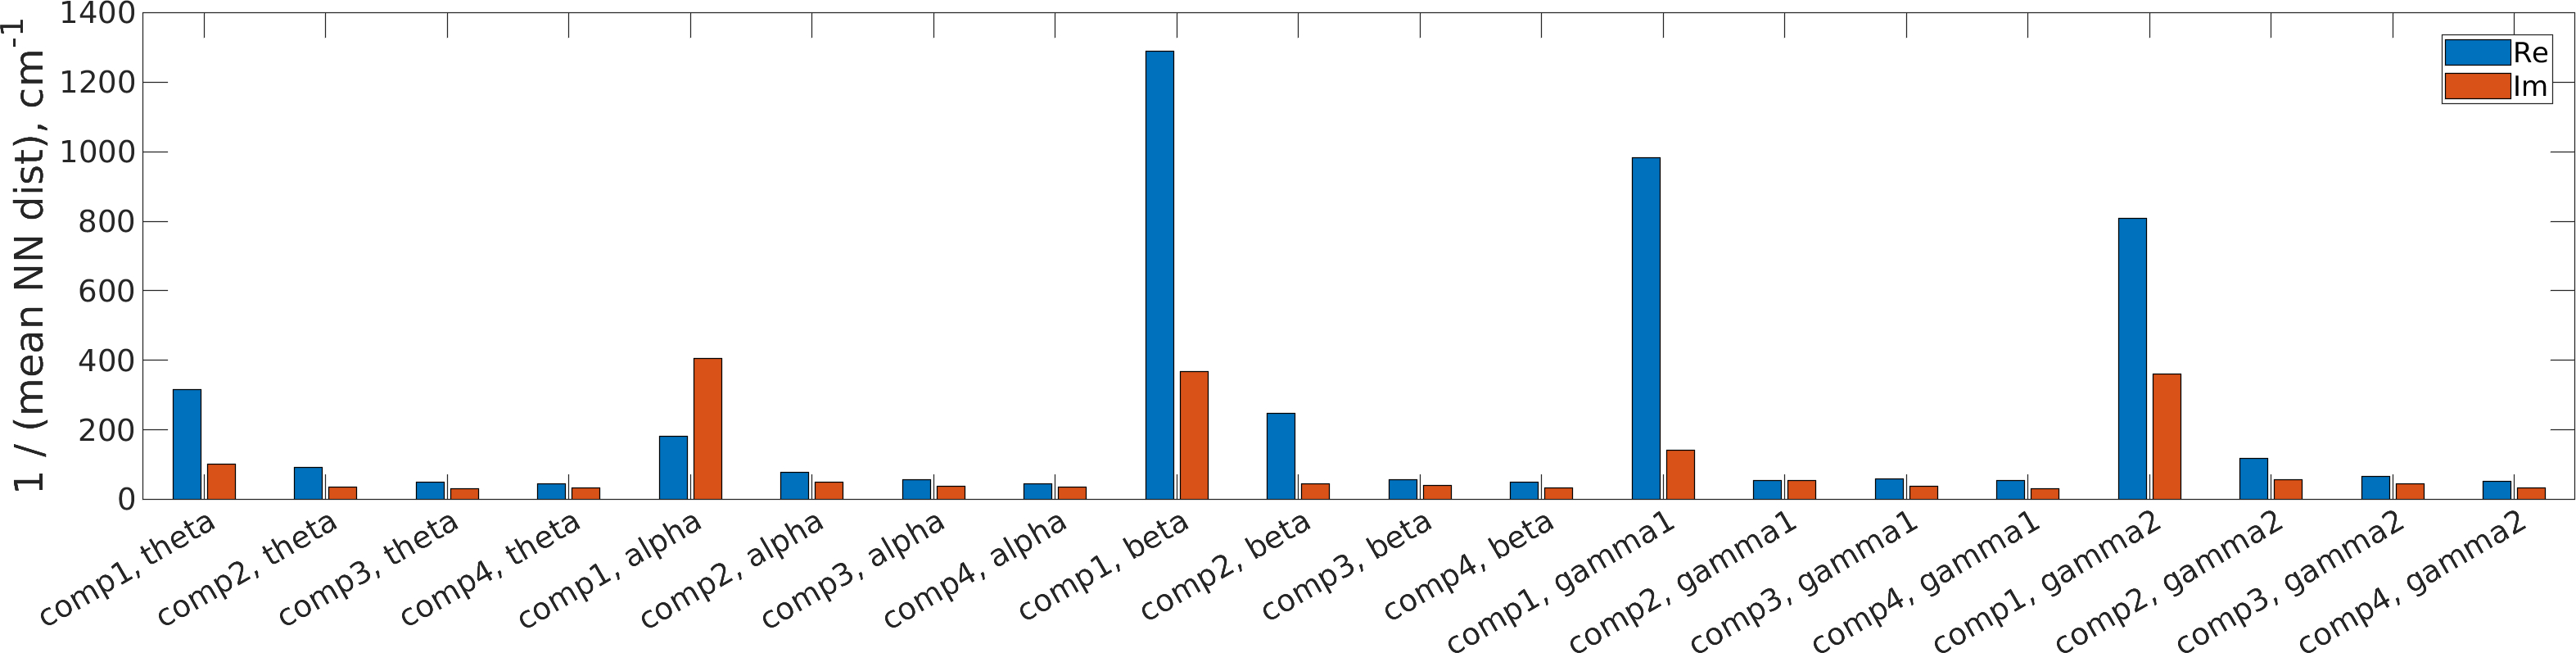
\includegraphics[width=1\textwidth]{../images/psiicos_paper/Figure10_hr.jpg}
 \caption{Полосы частот с наиболее воспроизводимыми сетями, определенными при помощи
 процедуры бутстрэпа.}\label{fig:10}
 Бутстрэп проводился последовательным выбором подмножества эпох, на котором
 вычислялся кросс-спектр, к которому затем применялась PSIICOS-проекция.
 Столбики на графике отображают индекс воспроизводимости, который вычислялся
 как обратное к среднему расстоянию до ближайшего соседа для каждой отдельной
 сети, найденной по мнимой и действительной спроецированной части кросс-спектра для четырех
 наиболее значимых главных компонент. Результаты для действительной части представлены
 синим цветом, а для мнимой~--- желтым.
 \end{figure} %Figure 10

 На графиках~\ref{fig:11},~\ref{fig:12},~\ref{fig:13} изображена пространственная
структура обнаруженных сетей для этих частотных диапазонов. Сети, узлы которых
оказывались ближе 1 сантиметра друг к другу, мы рисовали одним цветом. Перекрывающиеся сети
мы рисовали с увеличинным размером маркера и увеличенной толщиной линии. Прозрачность
линии мы меняли в зависимости от плотности сетей в кластере с учетом перекрытий.
Также для каждой воспроизводимой компоненты мы рисовали профиль ее временной активации
как правый собственный вектор сингулярного разложения соответствующей части временного
ряда кросс-спектра.

\begin{figure}
\centering
\text{Тета- (3--6 Гц) и альфа- (8--12 Гц) диапазоны}

 \begin{subfigure}[b]{0.4\textwidth}
 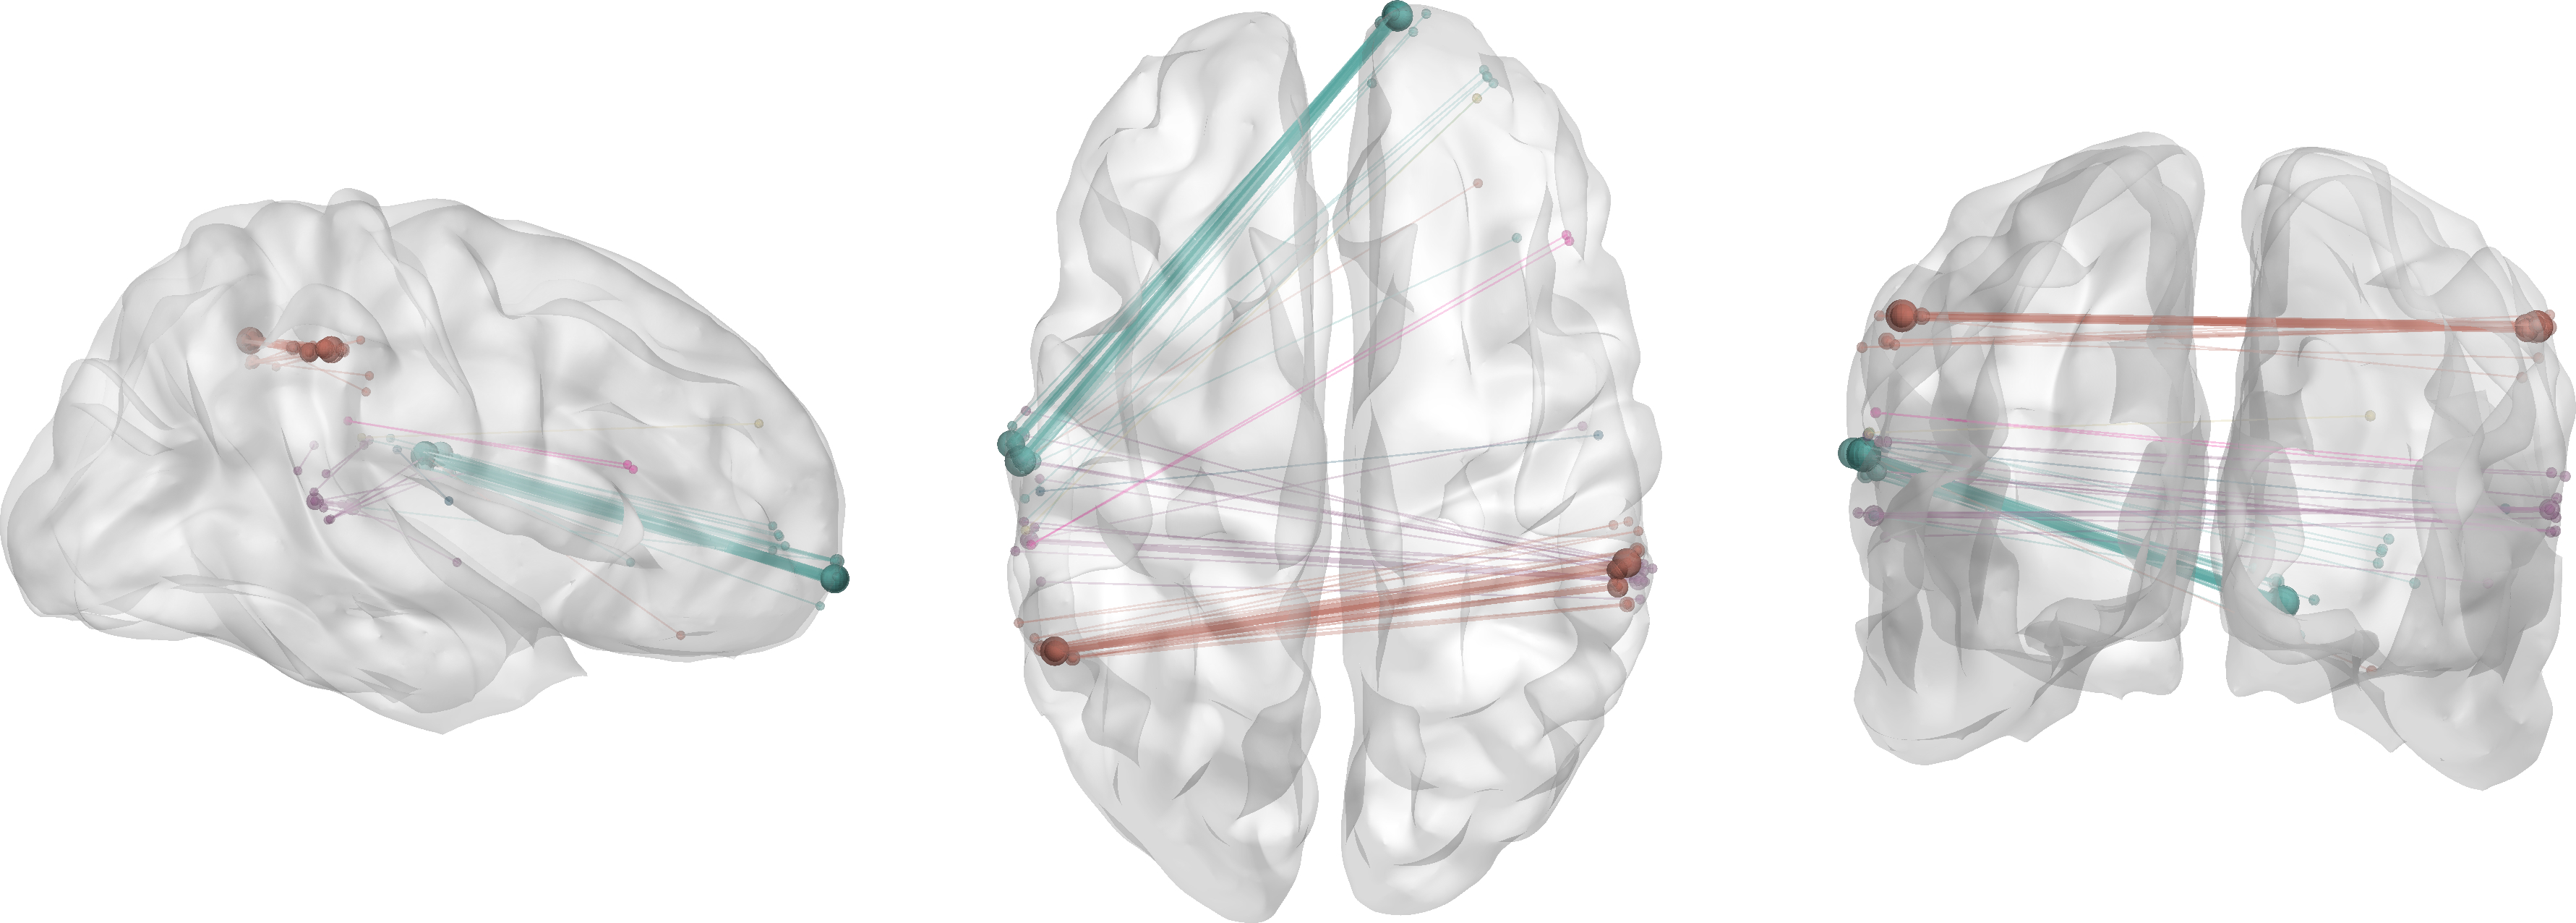
\includegraphics[width=\textwidth]{../images/psiicos_paper/Figure11_a1.jpg}
 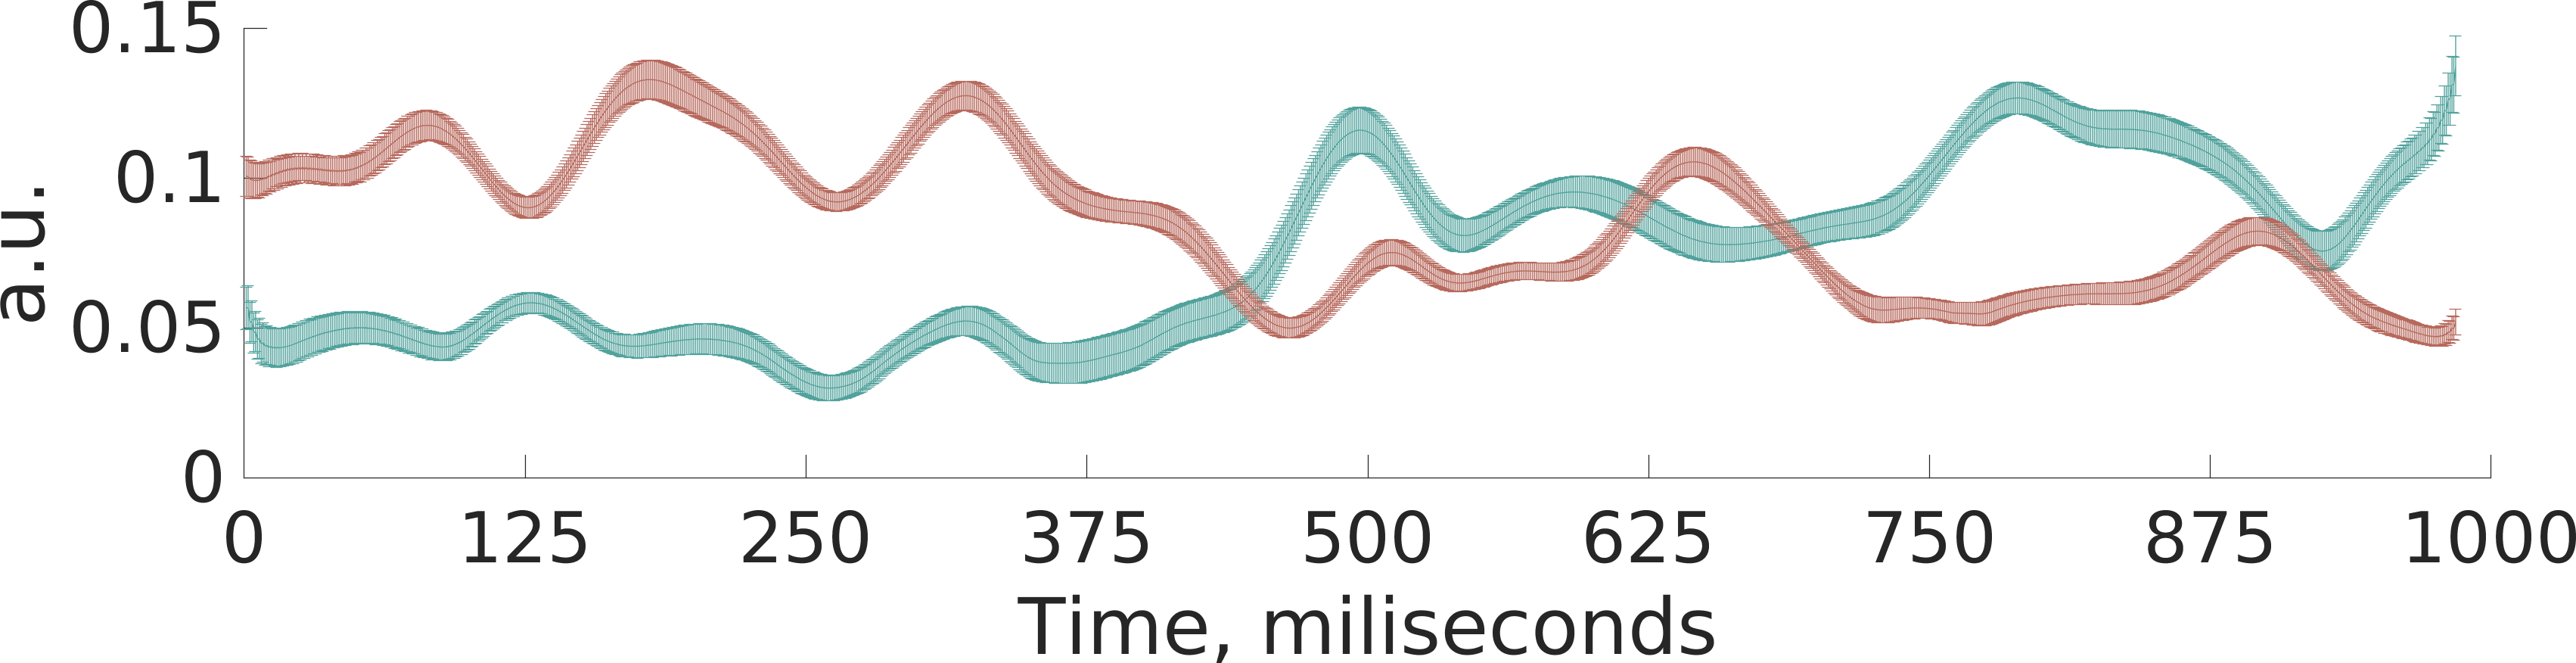
\includegraphics[width=\textwidth]{../images/psiicos_paper/Figure11_a2.jpg}
 \caption{Тета-диапазон, Re, сеть 1}\label{fig:11a}
 \end{subfigure}
 \hspace{1cm}
 \begin{subfigure}[b]{0.4\textwidth}
 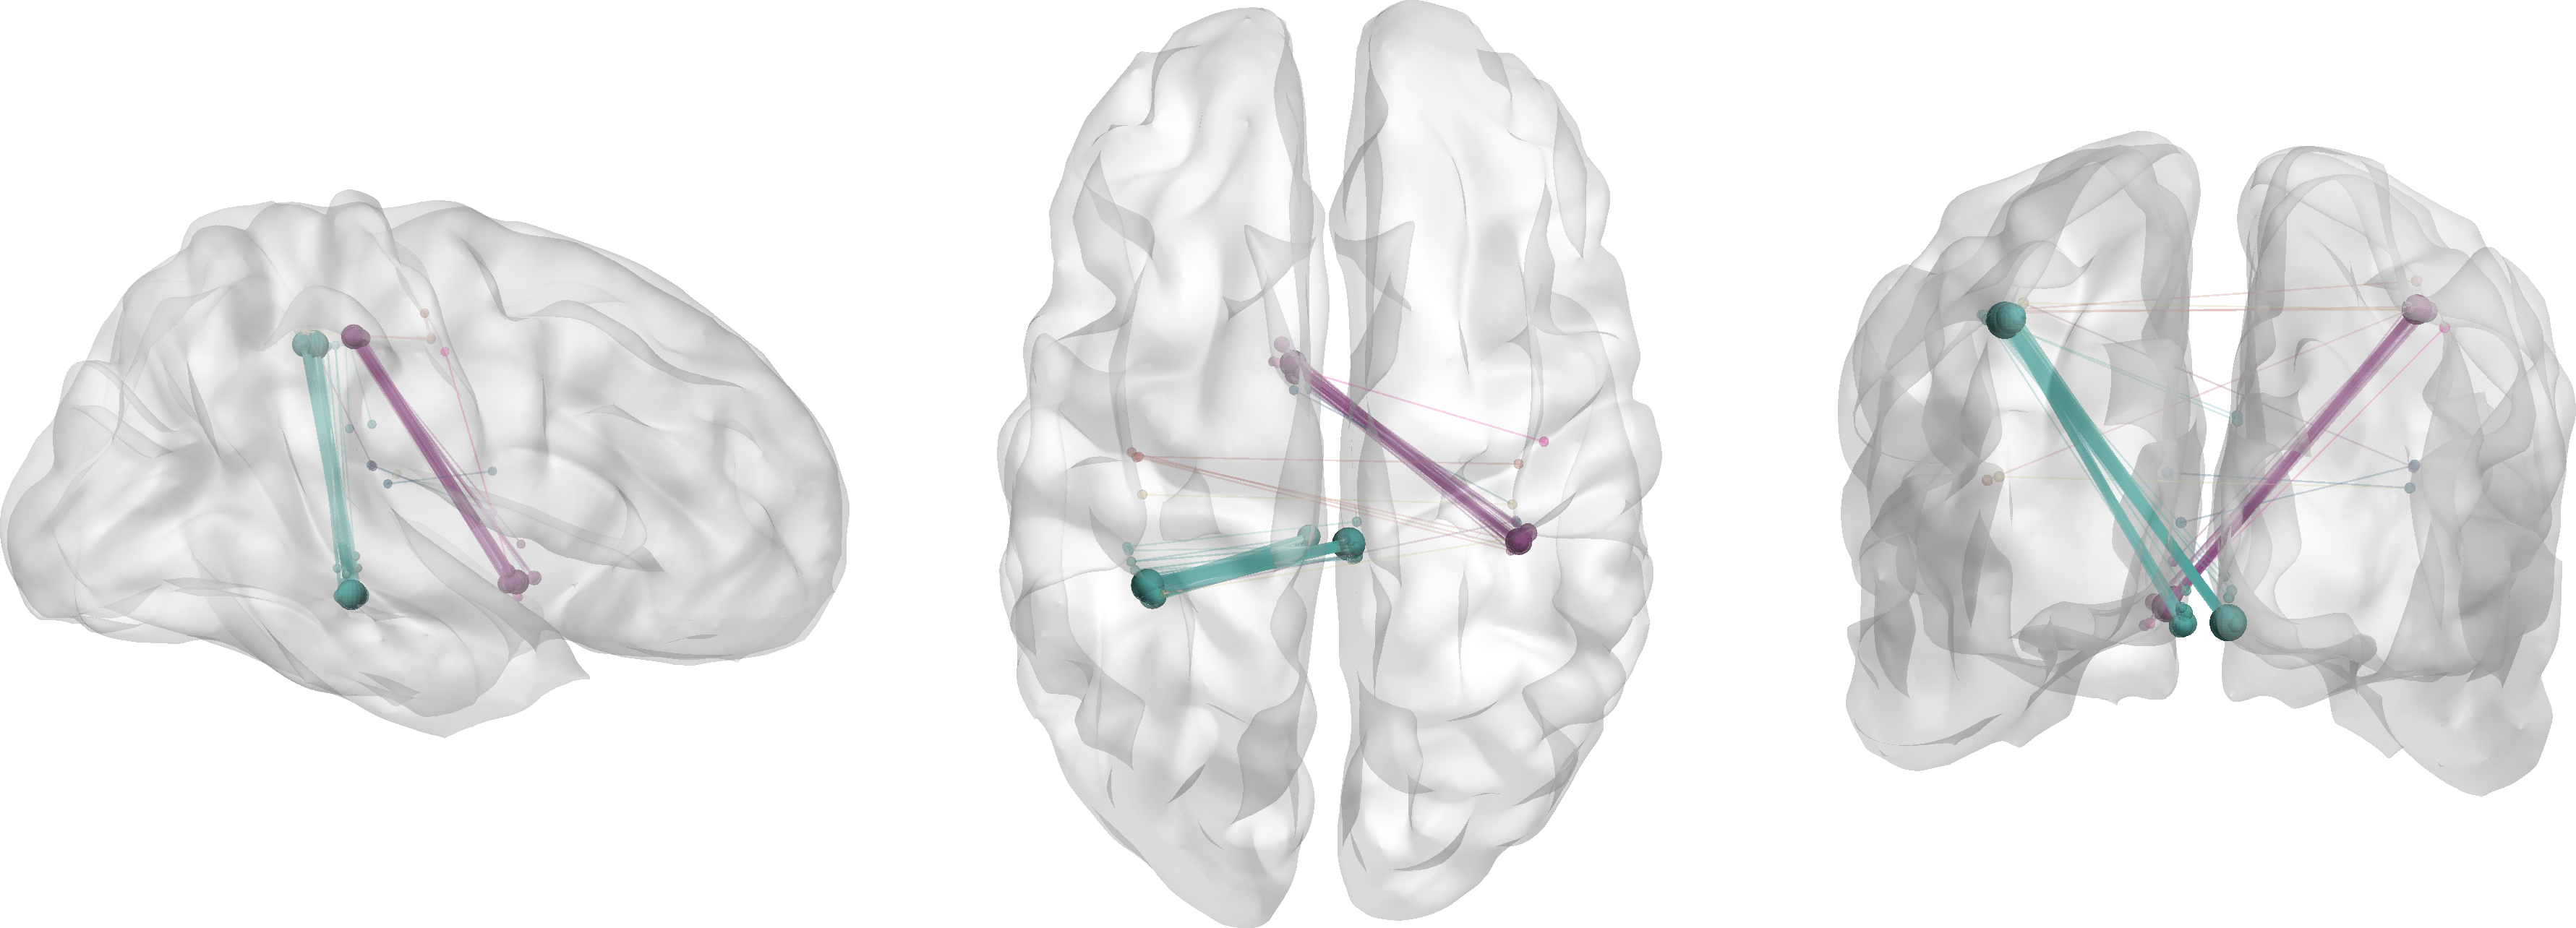
\includegraphics[width=\textwidth]{../images/psiicos_paper/Figure11_b1.jpg}
 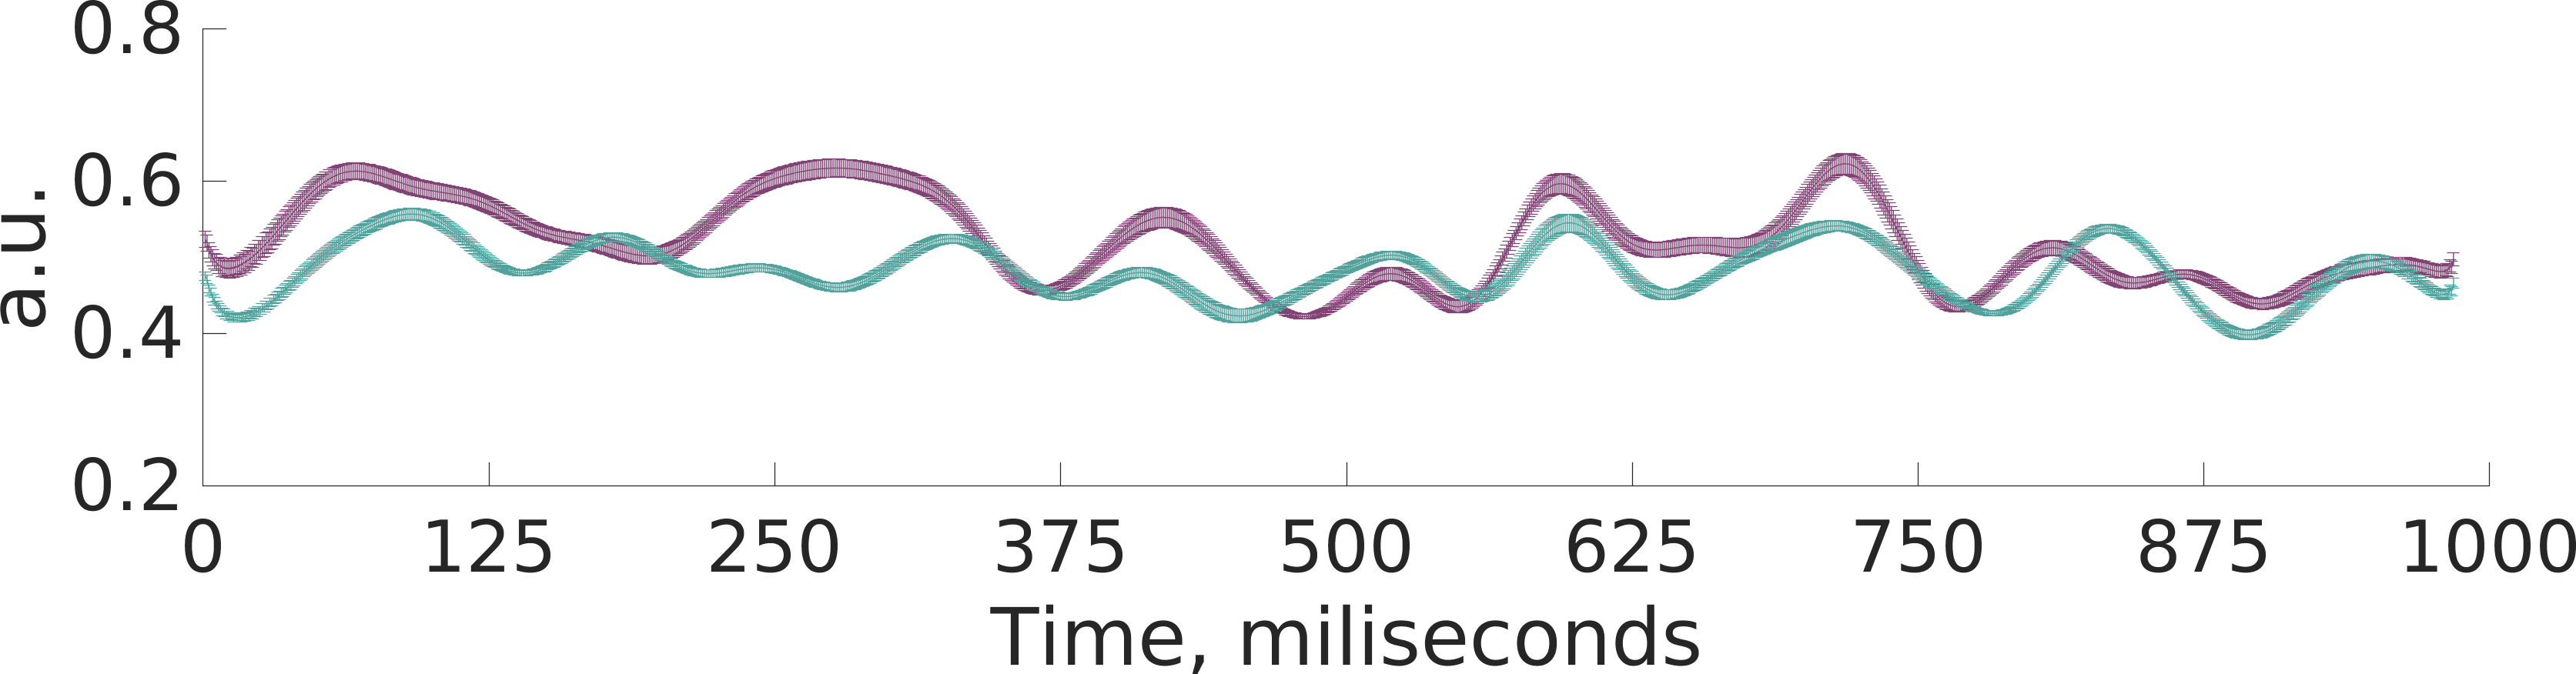
\includegraphics[width=\textwidth]{../images/psiicos_paper/Figure11_b2.jpg}
 \caption{Альфа-диапазон, Im, сеть 1}\label{fig:11b}
 \end{subfigure}
 \caption{Пространственная структура и временная динамика наиболее воспроизводимых сетей в диапазонах частот тета (3--6 Гц) и альфа (8--12 Гц)}\label{fig:11}
\end{figure} % figure 11

Анализ действительной части кросс-спектра показывает наличие следующих сетей с преимущественно
малыми фазовыми задержками. В тета-диапазоне (рис.~\ref{fig:11}) мы видим сети,
соединяющие правую орбито-фронтальную кору, вовлеченную в сенсорную интеграцию, с левым
билатеральным височно-теменным узлом, про который известно, что он активен при воображении
движения~(\cite{Hanakawa2008}). Также мы видим кросс-латеральную сеть, соединяющую два
теменных отдела.

В бета-диапазоне мы видим механистически правдоподобную кросс-латеральную связь
между вентральным зрительным путем и зоной репрезентации руки в моторной
области правого полушария. Дополнительно мы наблюдаем взаимодействие между
зонами представительства руки сенсомоторной области правого полушария и
соматосенсорной области левого, рис.~\ref{fig:12}, что частично
согласуется с наблюдениями, описанными в статье~\cite{Lamm2007} и соотносится
с профилями функциональной коннективности, описанными в  фМРТ-исследовании
воображаемых вращений~\cite{Striem-Amit2017}. Наконец, мы обнаружили взаимодействие
зоны представительства руки в моторной области правого полушария с височным полюсом
левого полушария в гамма-диапазоне, рис.~\ref{fig:13a}, а также с
орбито-фронтальной зоной левого полушария в верхнем гамма-диапазоне, рис.~\ref{fig:13b}.
Правдоподобность этих наблюдений подкреплена предполагаемой
ролью височного полюса левого полушария, в которую входит ``\ldots визуальное различение
двумерных изображений и мнемоническая функция соотнесения и научения'' (\cite{Dupont2002}).

\begin{figure}
\centering
\text{Бета-диапазон (16--24 Гц)}

 \begin{subfigure}[b]{0.4\textwidth}
 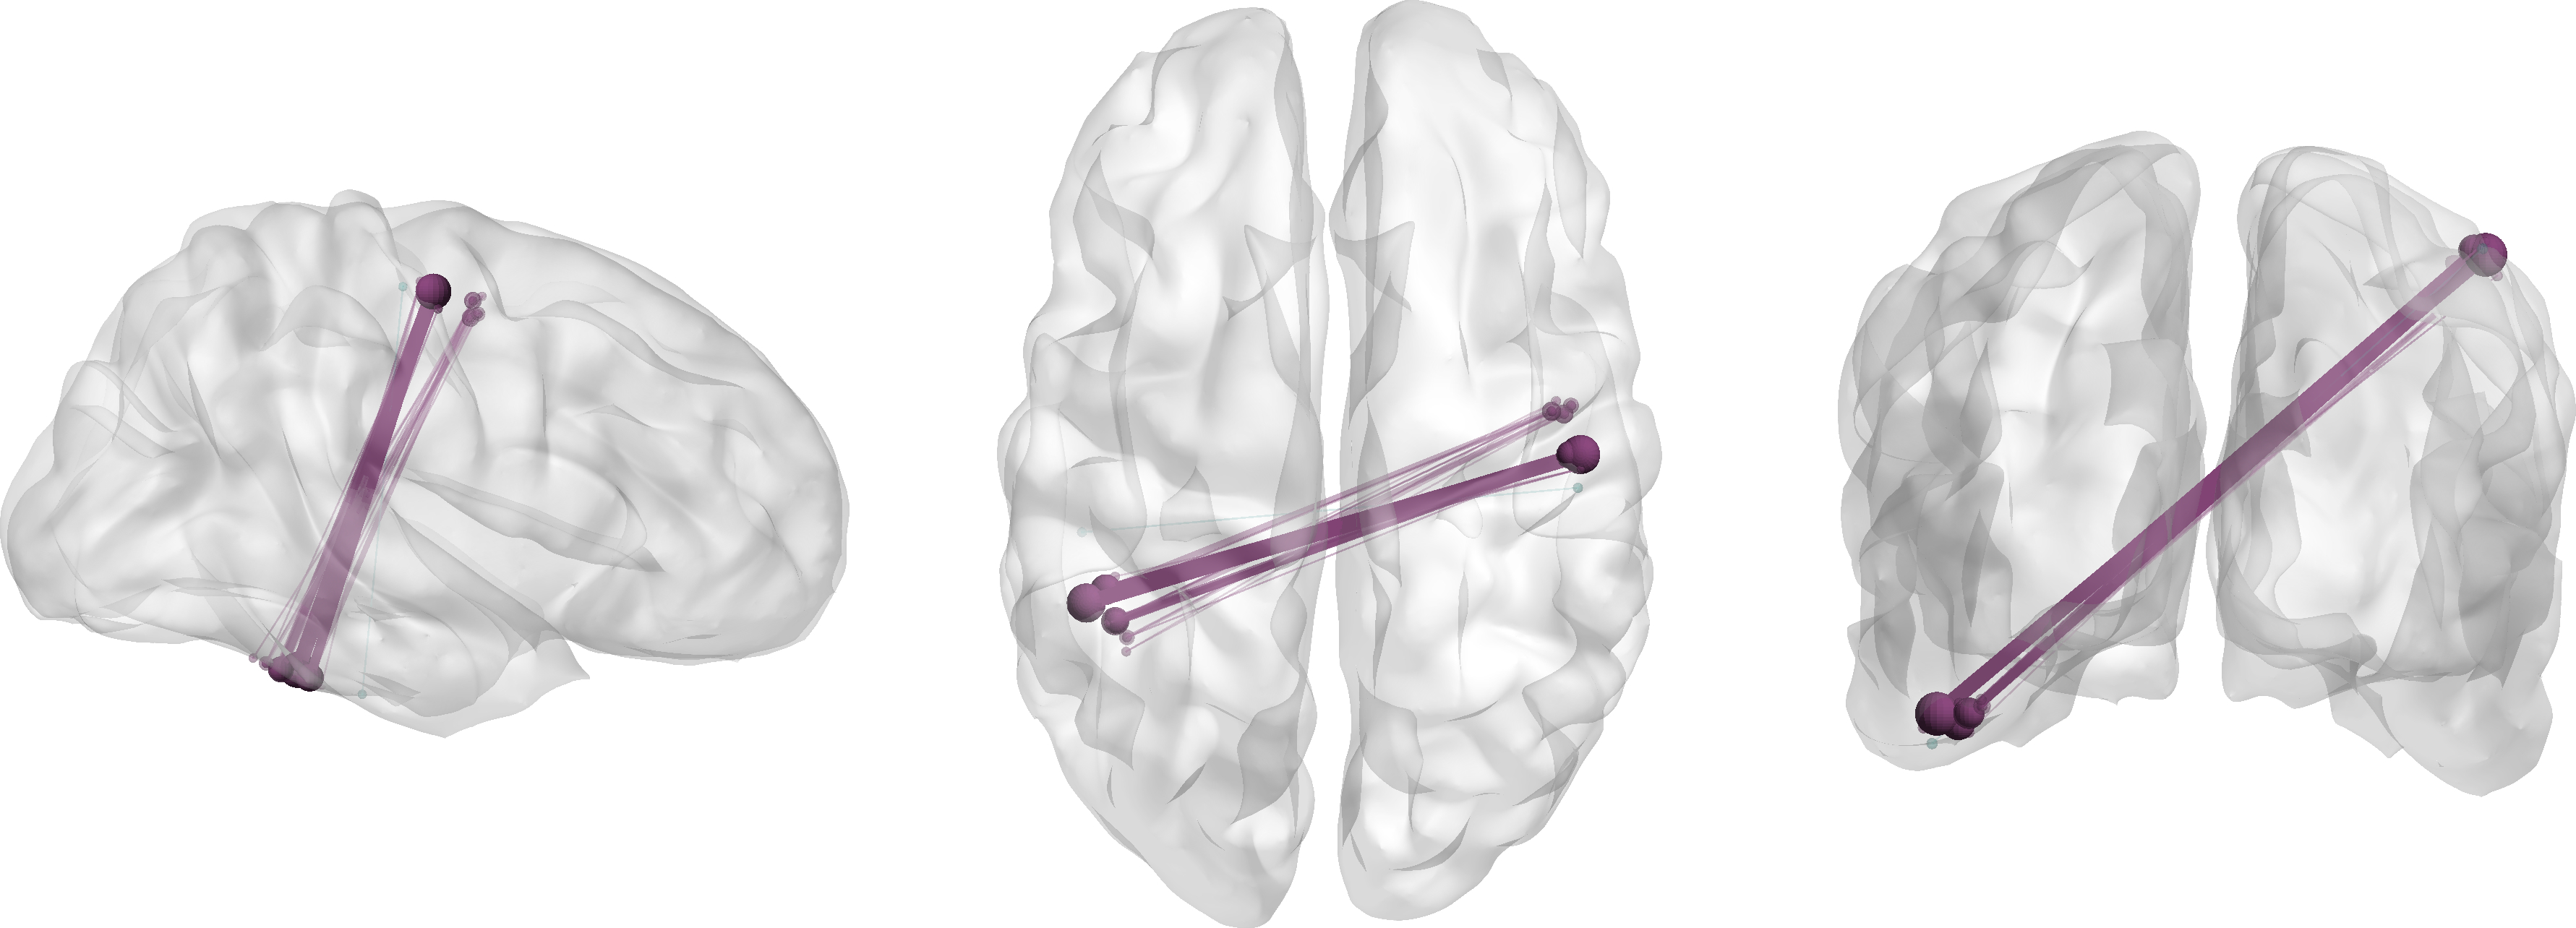
\includegraphics[width=\textwidth]{../images/psiicos_paper/Figure12_a1.jpg}
 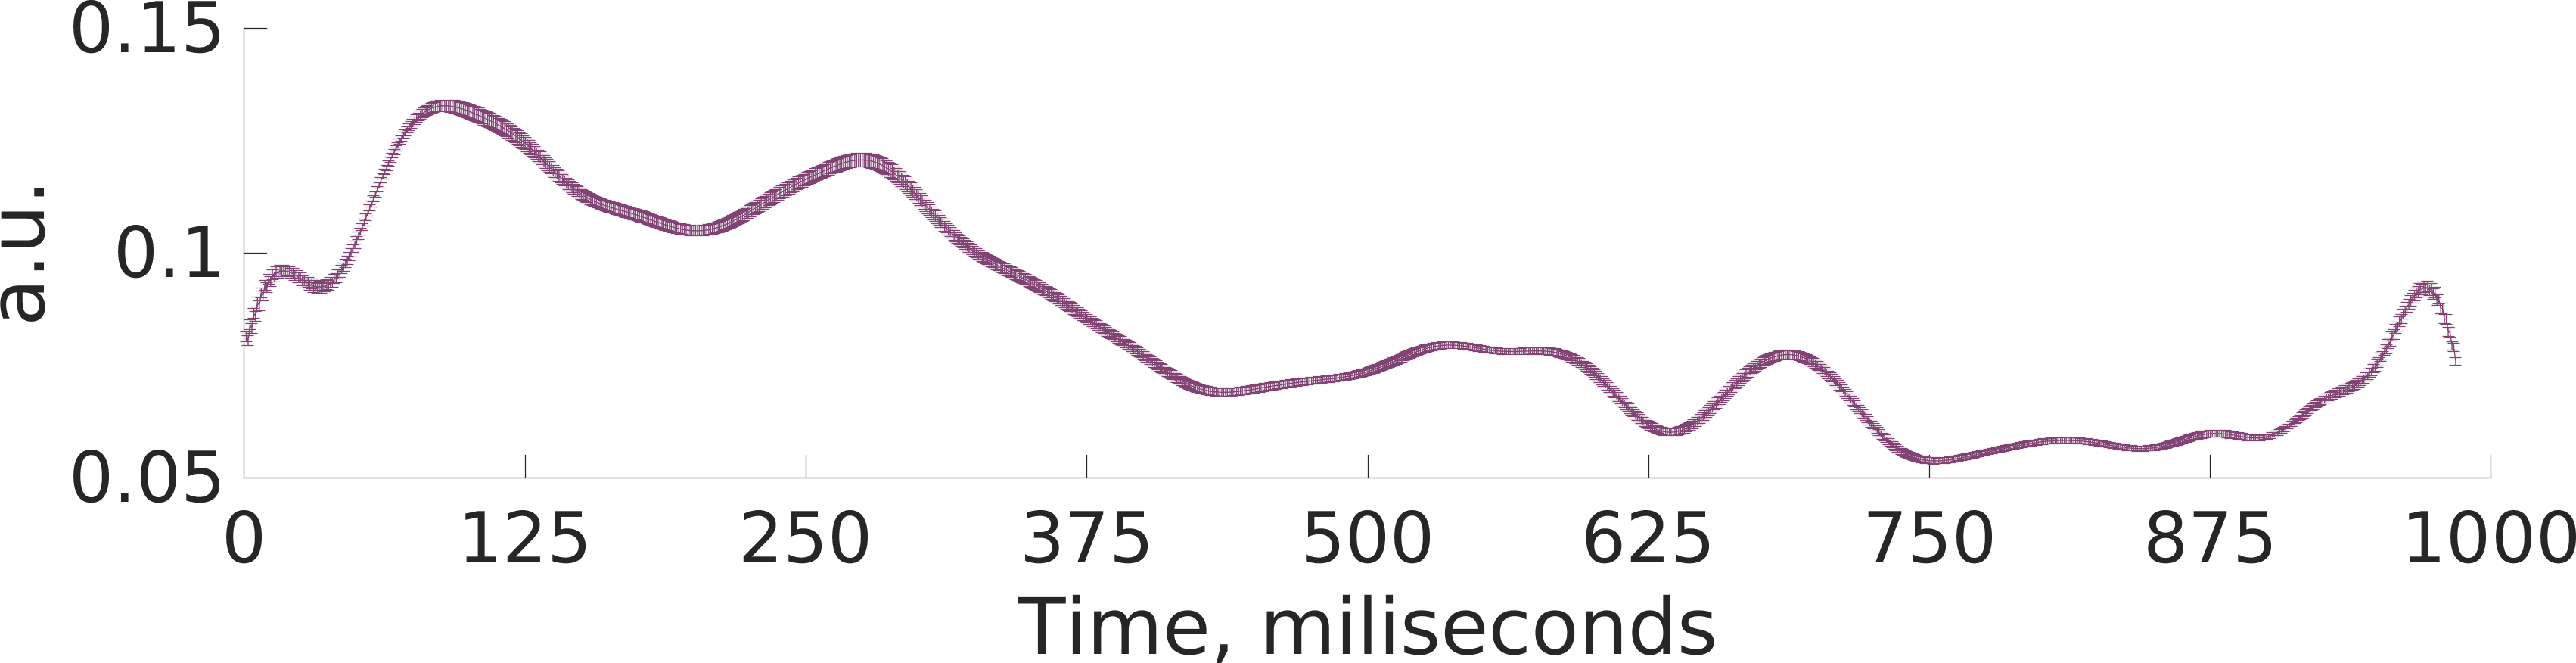
\includegraphics[width=\textwidth]{../images/psiicos_paper/Figure12_a2.jpg}
 \caption{Re, сеть 1}\label{fig:12a}
 \end{subfigure}
 \hspace{1cm}
 \begin{subfigure}[b]{0.4\textwidth}
 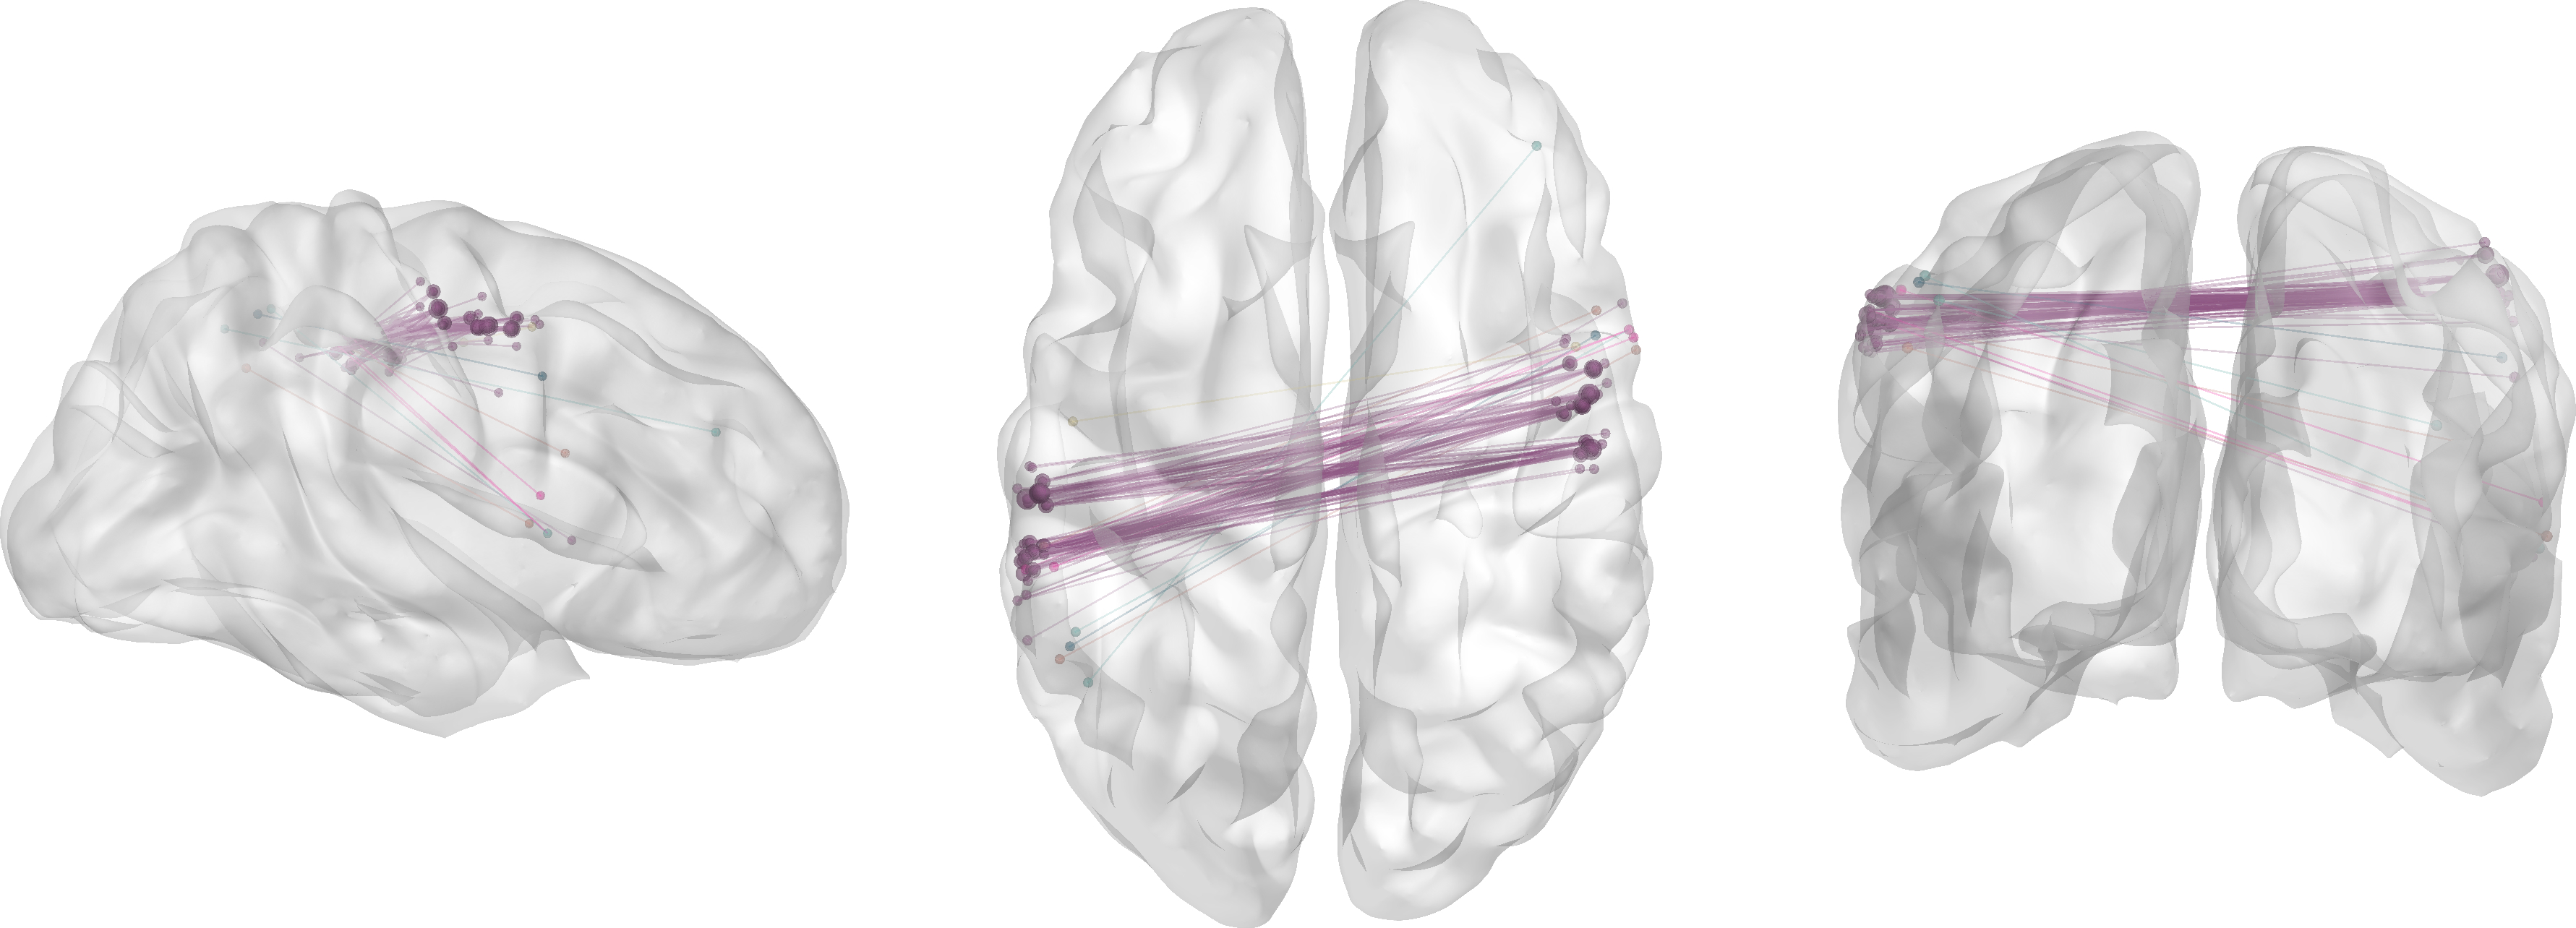
\includegraphics[width=\textwidth]{../images/psiicos_paper/Figure12_b1.jpg}
 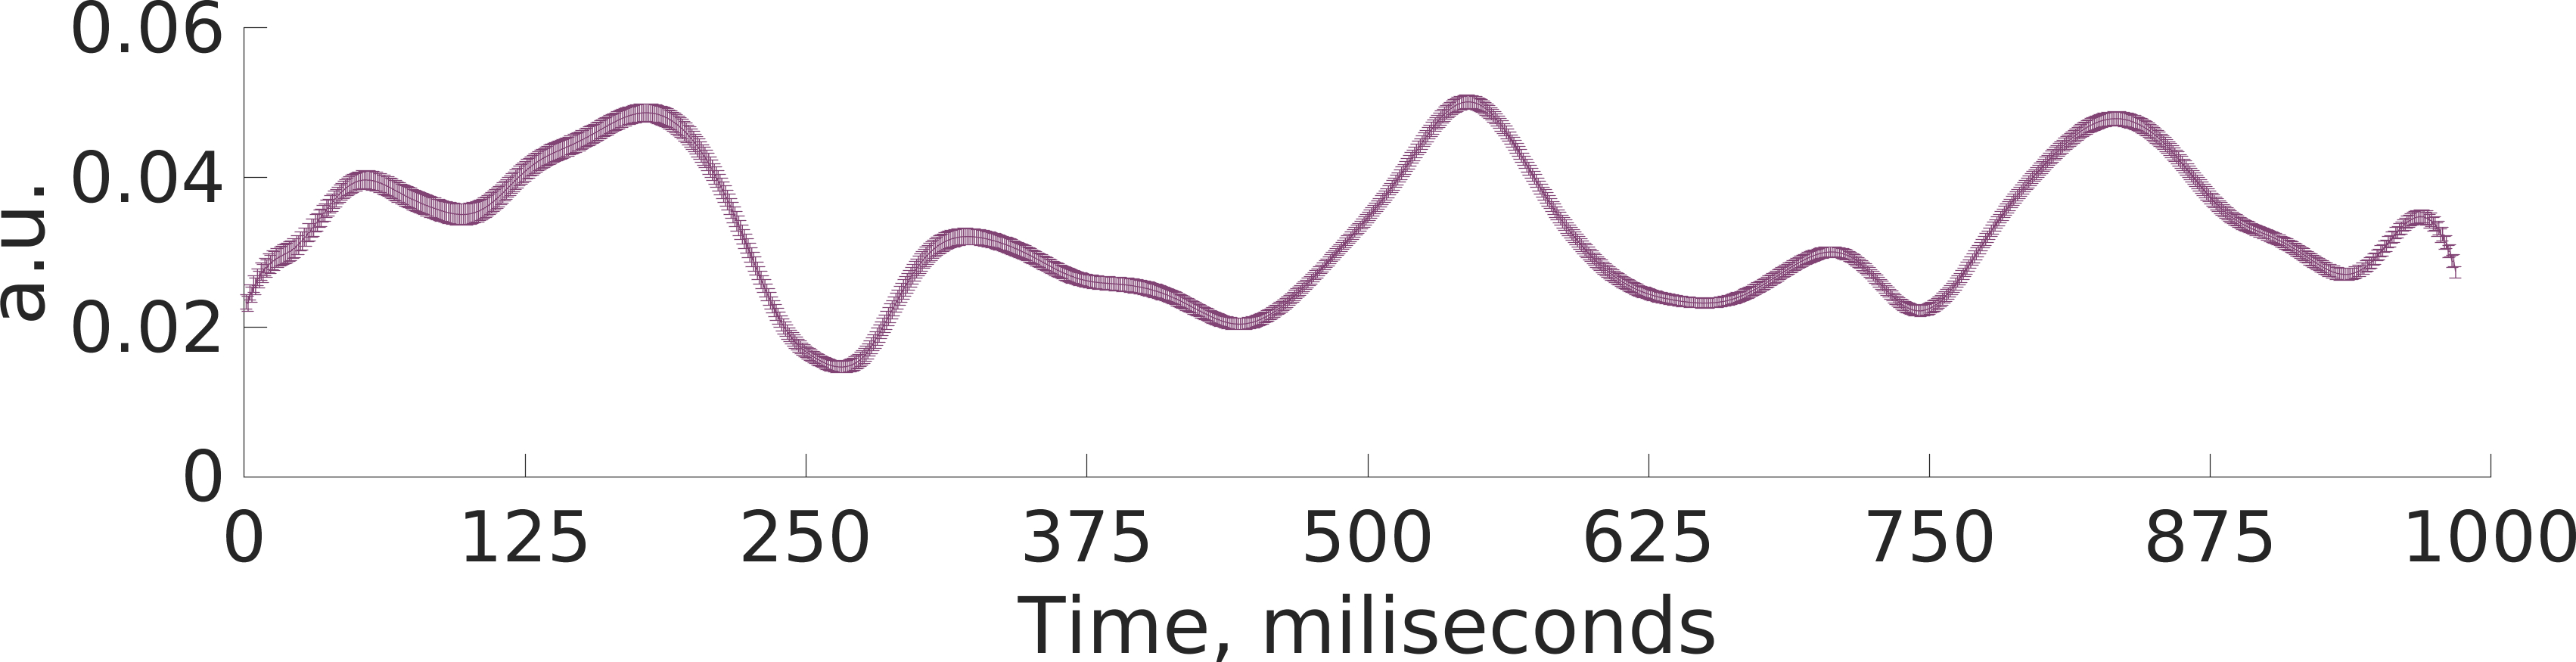
\includegraphics[width=\textwidth]{../images/psiicos_paper/Figure12_b2.jpg}
 \caption{Re, сеть 2}\label{fig:12b}
 \end{subfigure}
 \begin{subfigure}[b]{0.4\textwidth}
 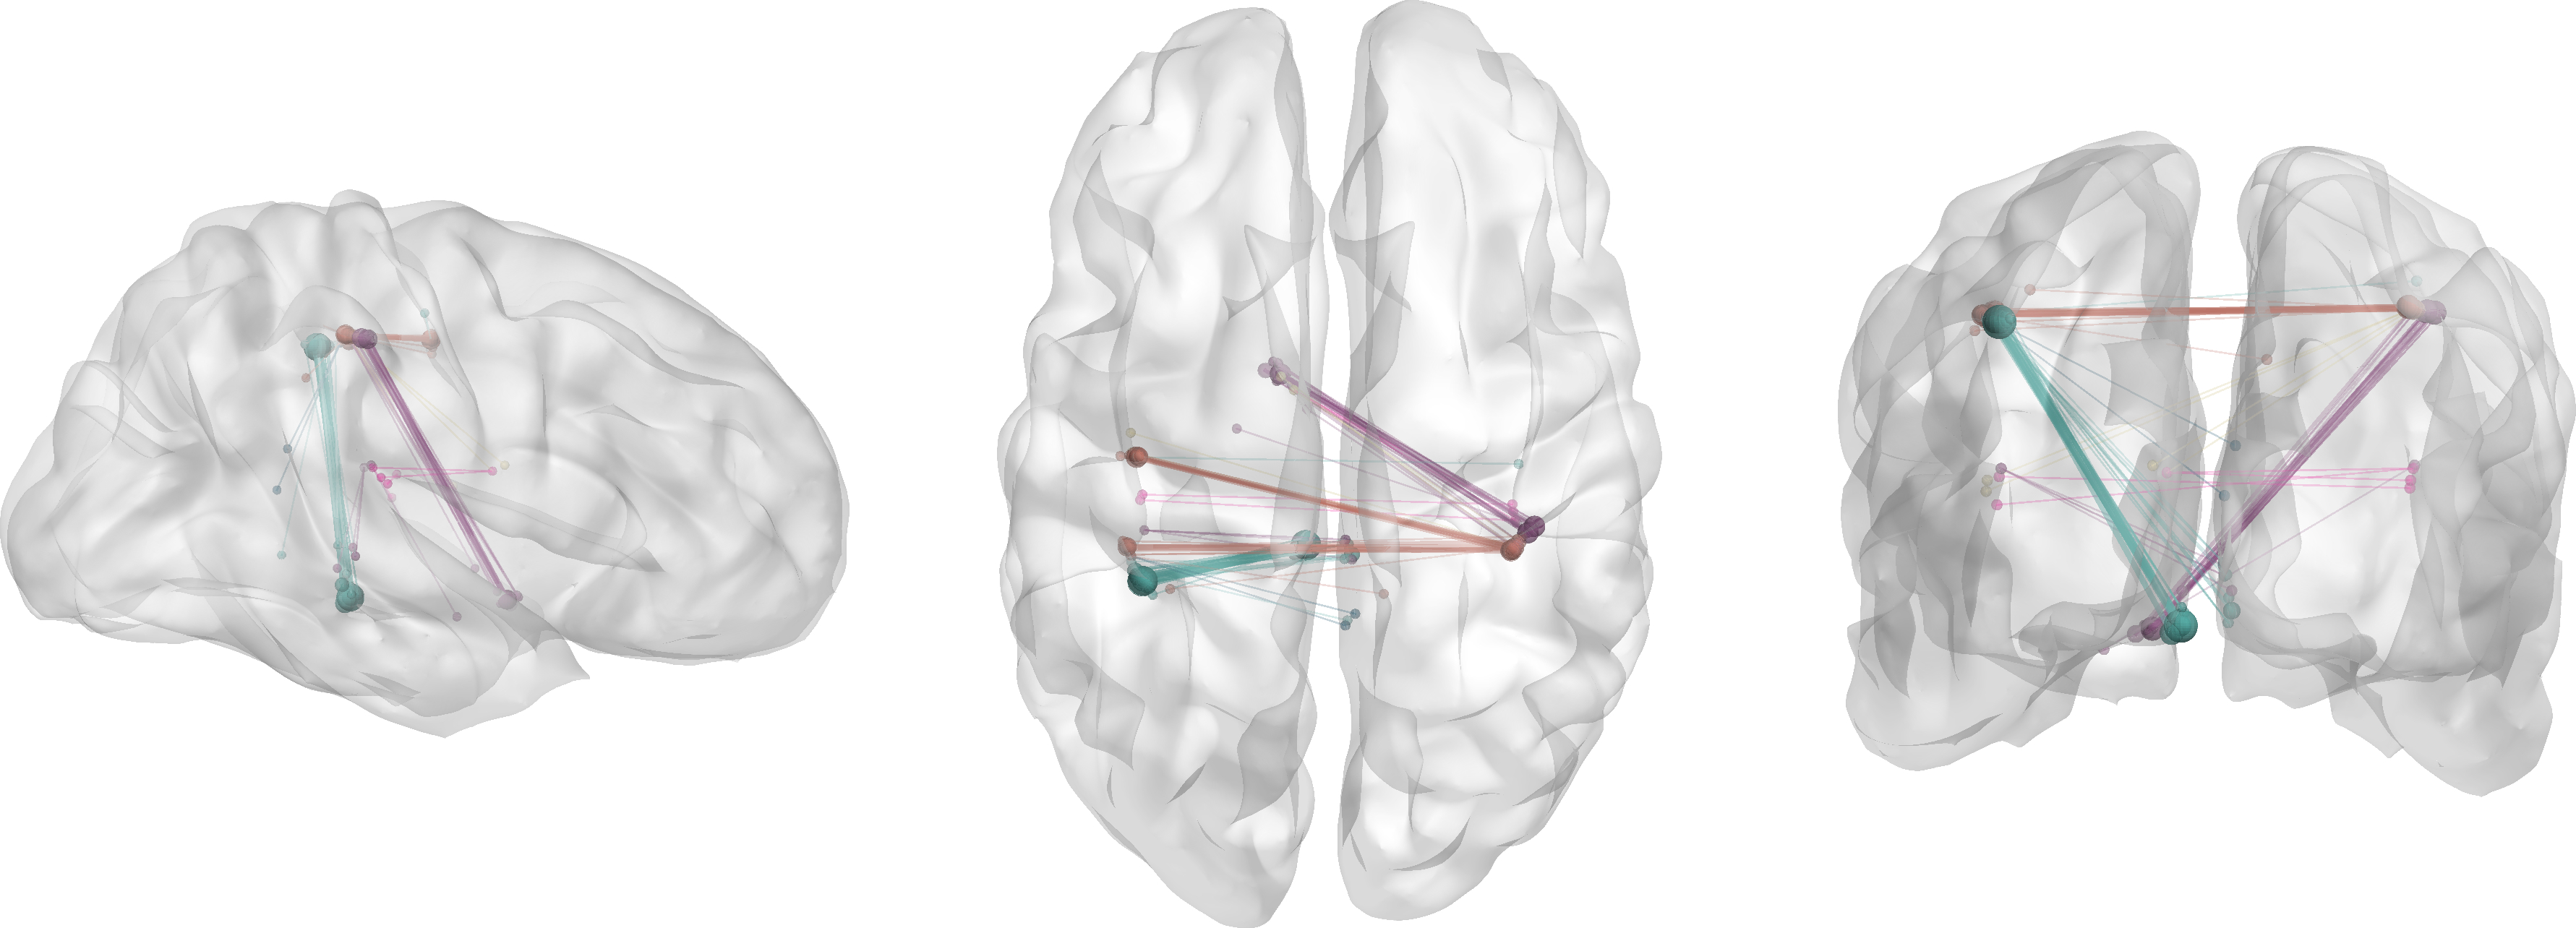
\includegraphics[width=\textwidth]{../images/psiicos_paper/Figure12_c1.jpg}
 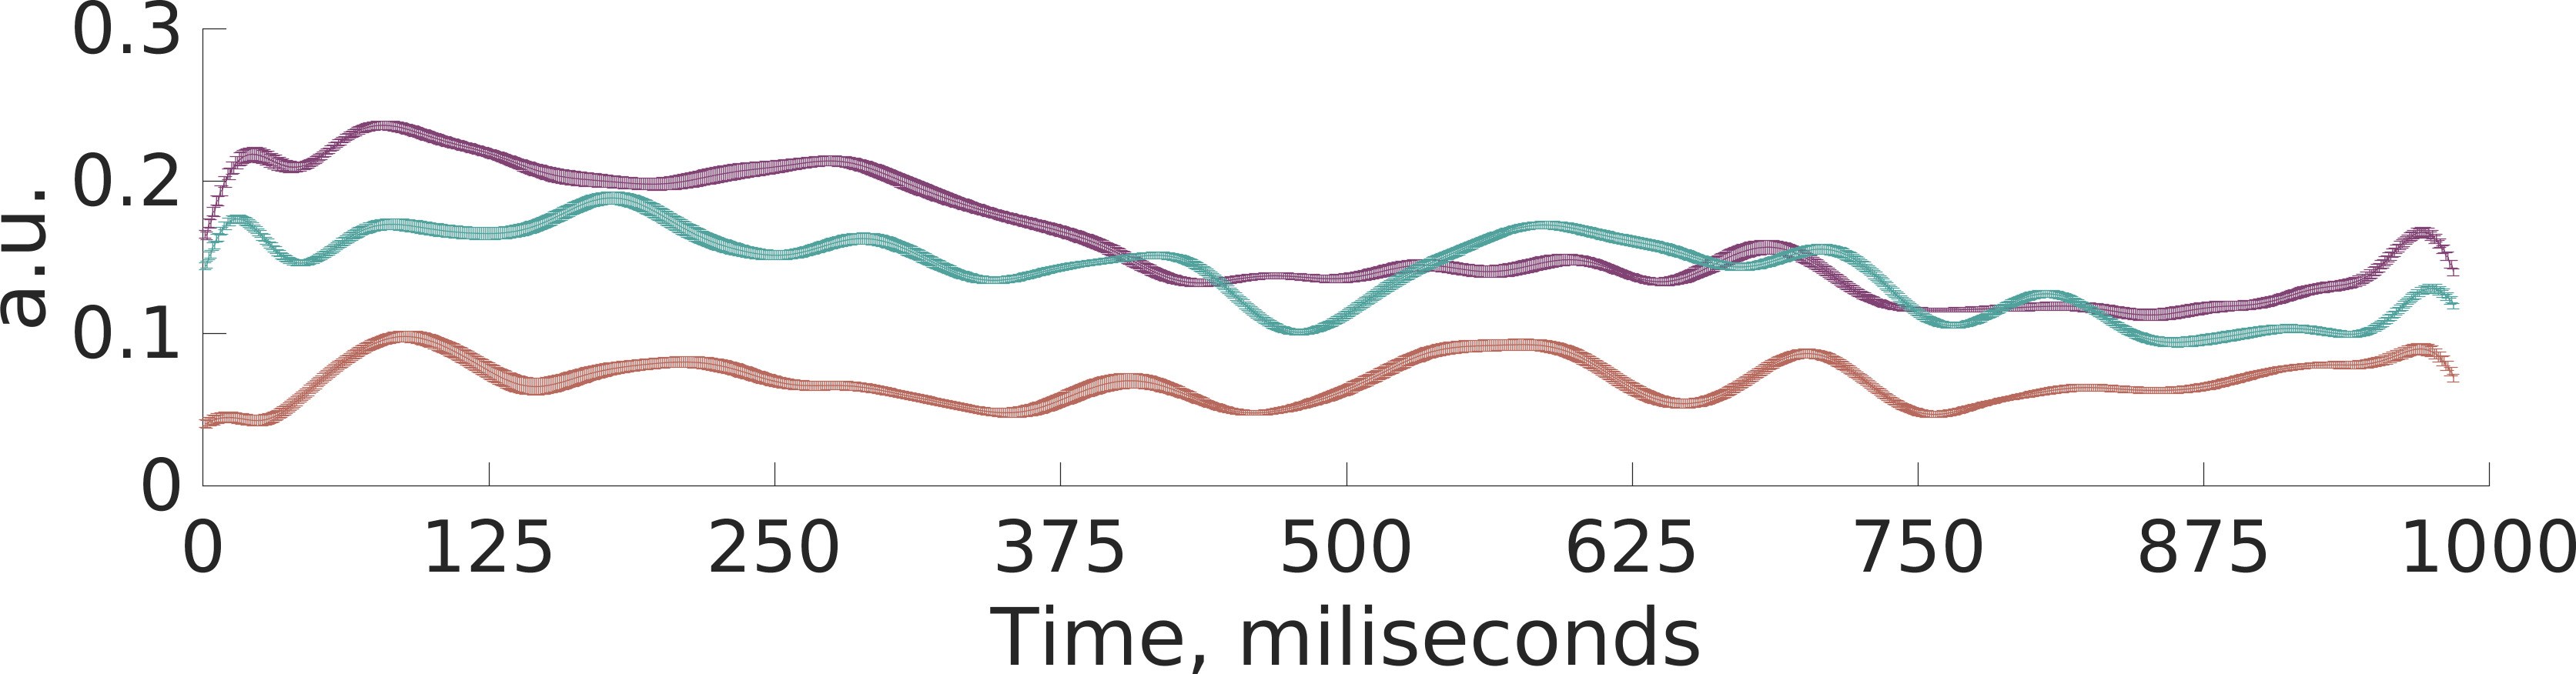
\includegraphics[width=\textwidth]{../images/psiicos_paper/Figure12_c2.jpg}

 \caption{Im, сеть 1}\label{fig:12c}
 \end{subfigure}
 \caption{Пространственная структура и временная динамика наиболее воспроизводимых сетей в бета-диапазоне (16--24 Гц)}\label{fig:12}
\end{figure} %figure 12

\begin{figure}
\centering
\text{Нижний (30--60 Гц) и верхний (65--85 Hz) гамма-диапазоны}

 \begin{subfigure}[b]{0.4\textwidth}
 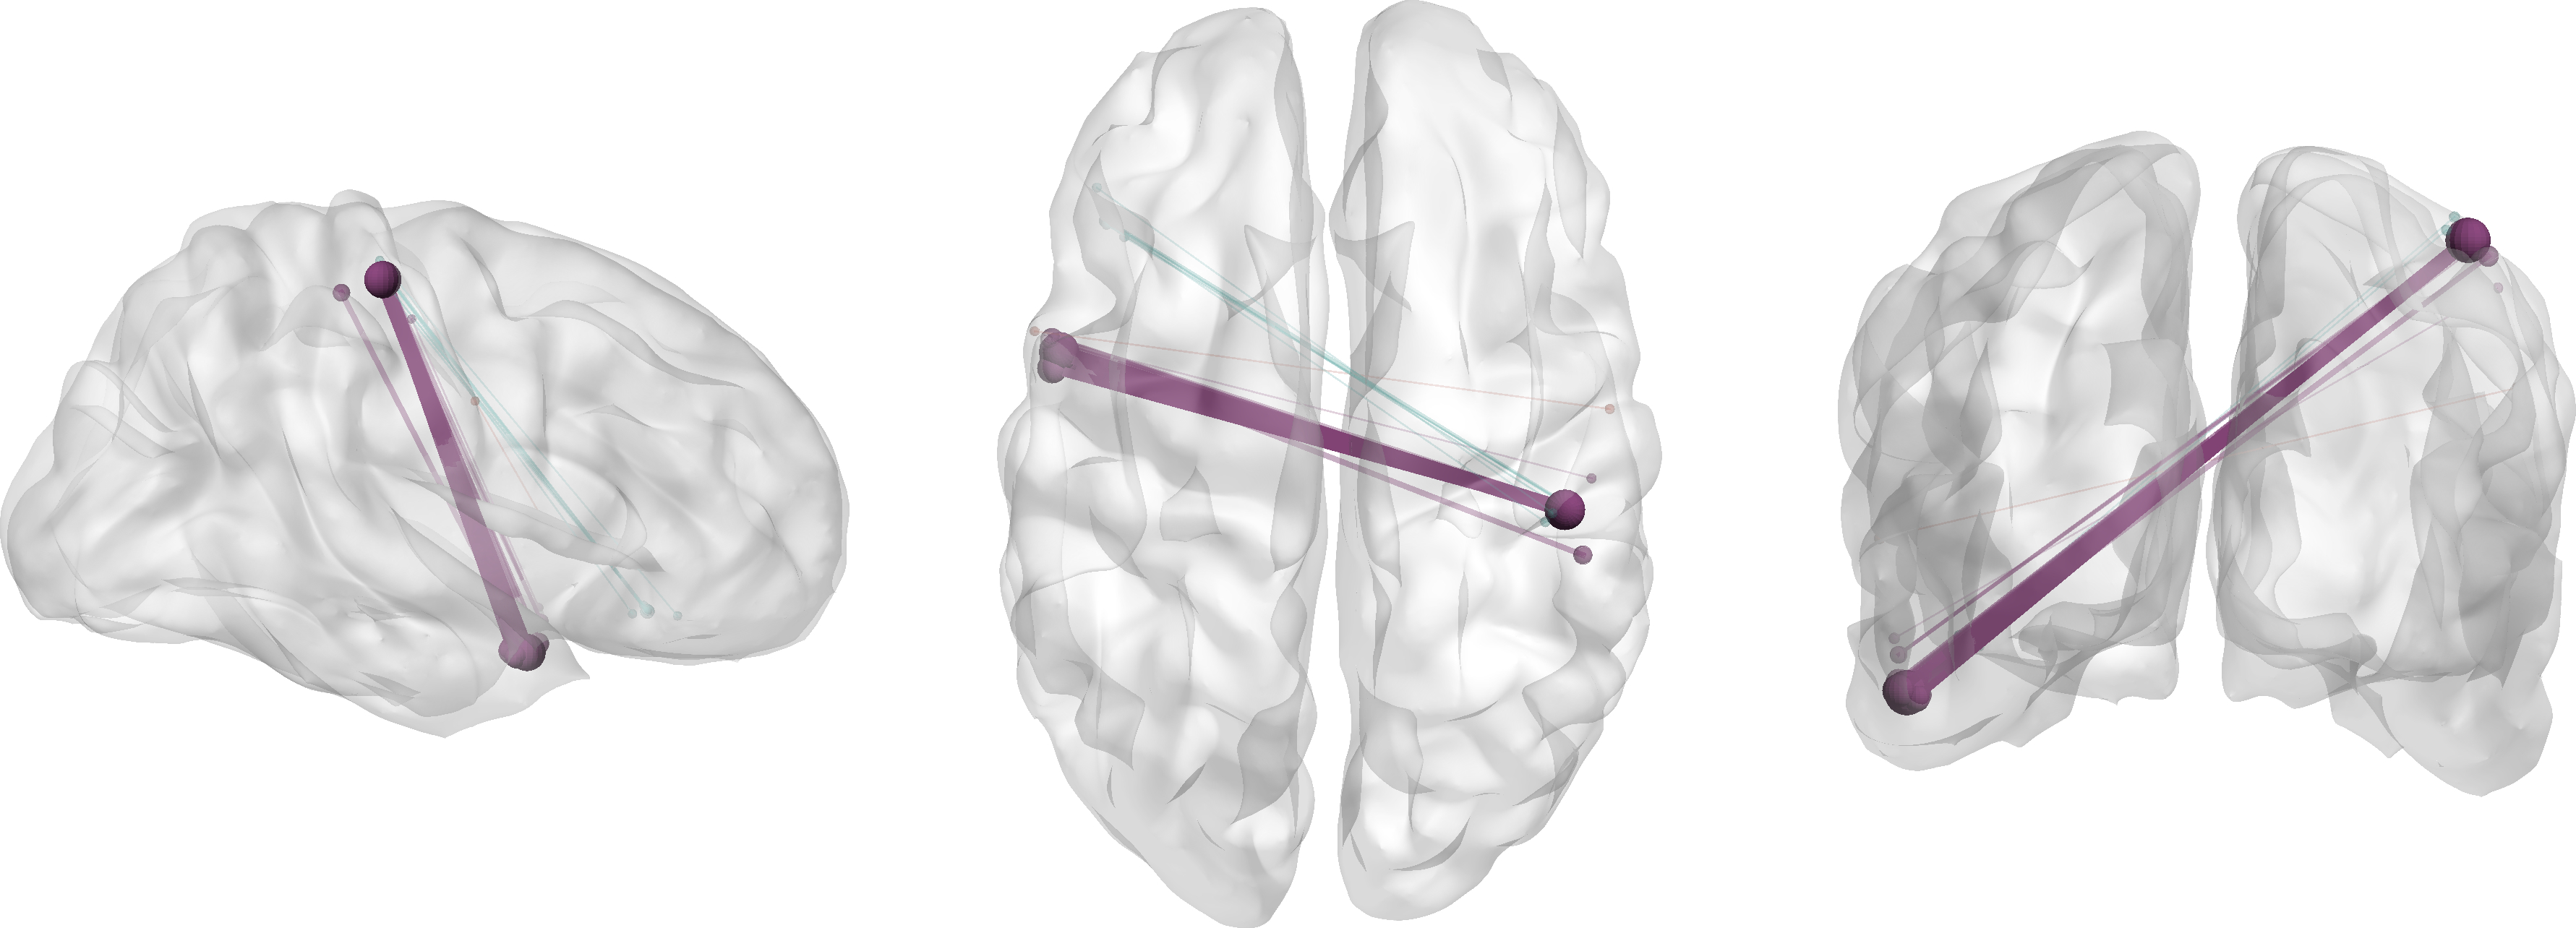
\includegraphics[width=\textwidth]{../images/psiicos_paper/Figure13_a1.jpg}
 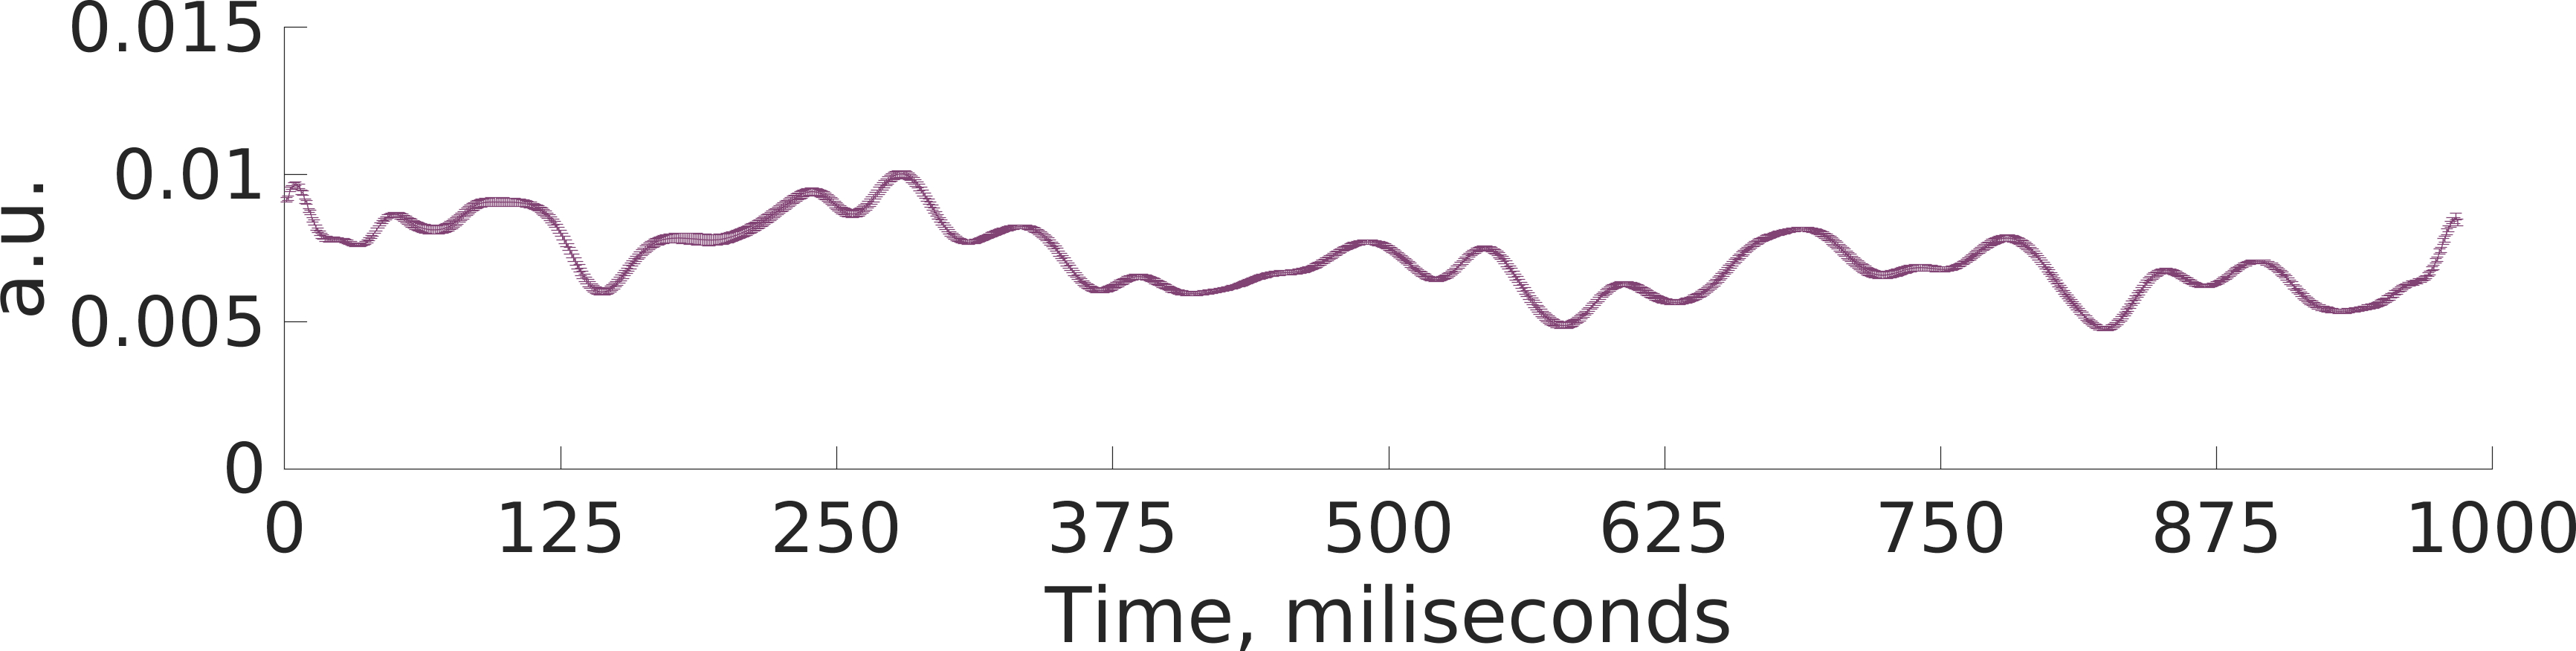
\includegraphics[width=\textwidth]{../images/psiicos_paper/Figure13_a2.jpg}
 \caption{Ниж. гамма-диапазон, Re, сеть 1}\label{fig:13a}
 \end{subfigure}
 \hspace{1cm}
 \begin{subfigure}[b]{0.4\textwidth}
 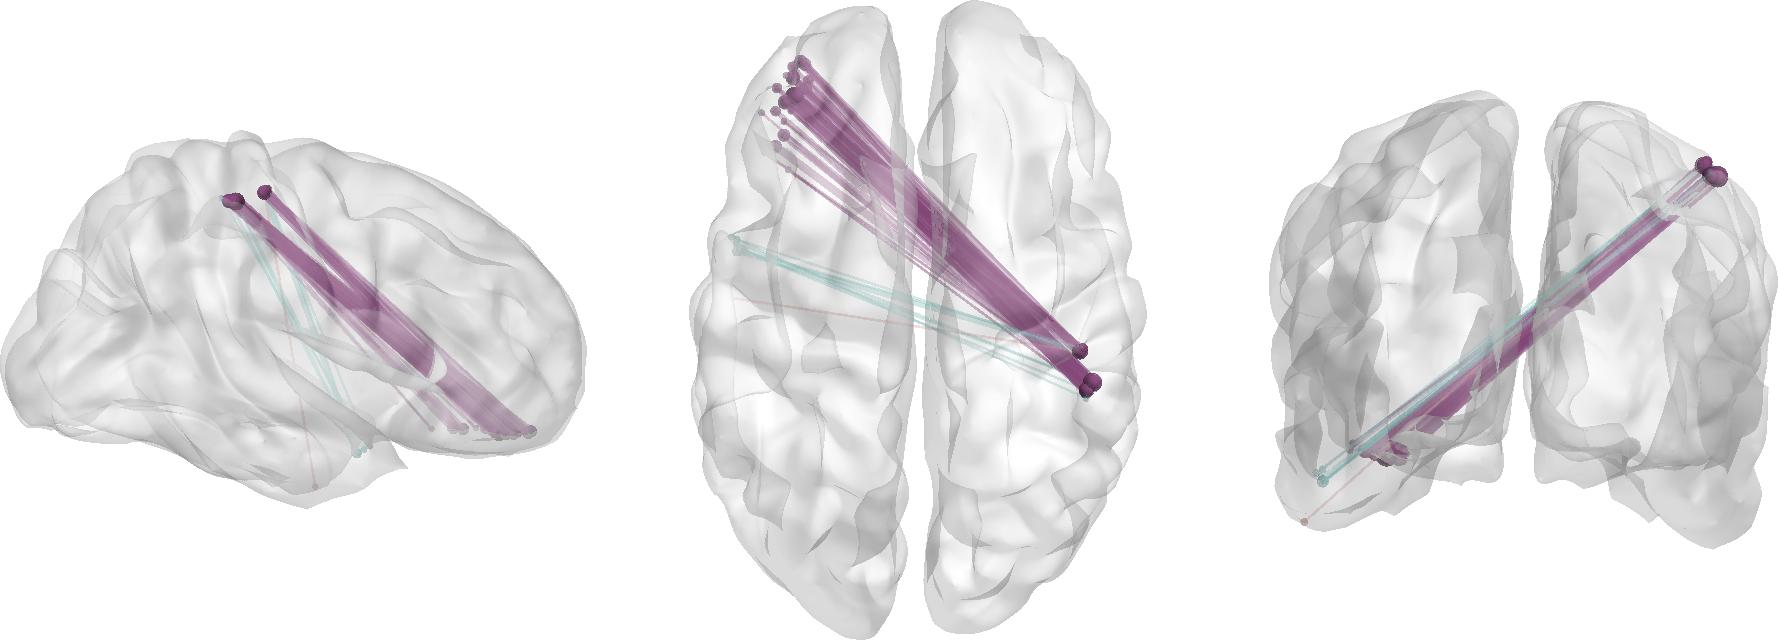
\includegraphics[width=\textwidth]{../images/psiicos_paper/Figure13_b1.jpg}
 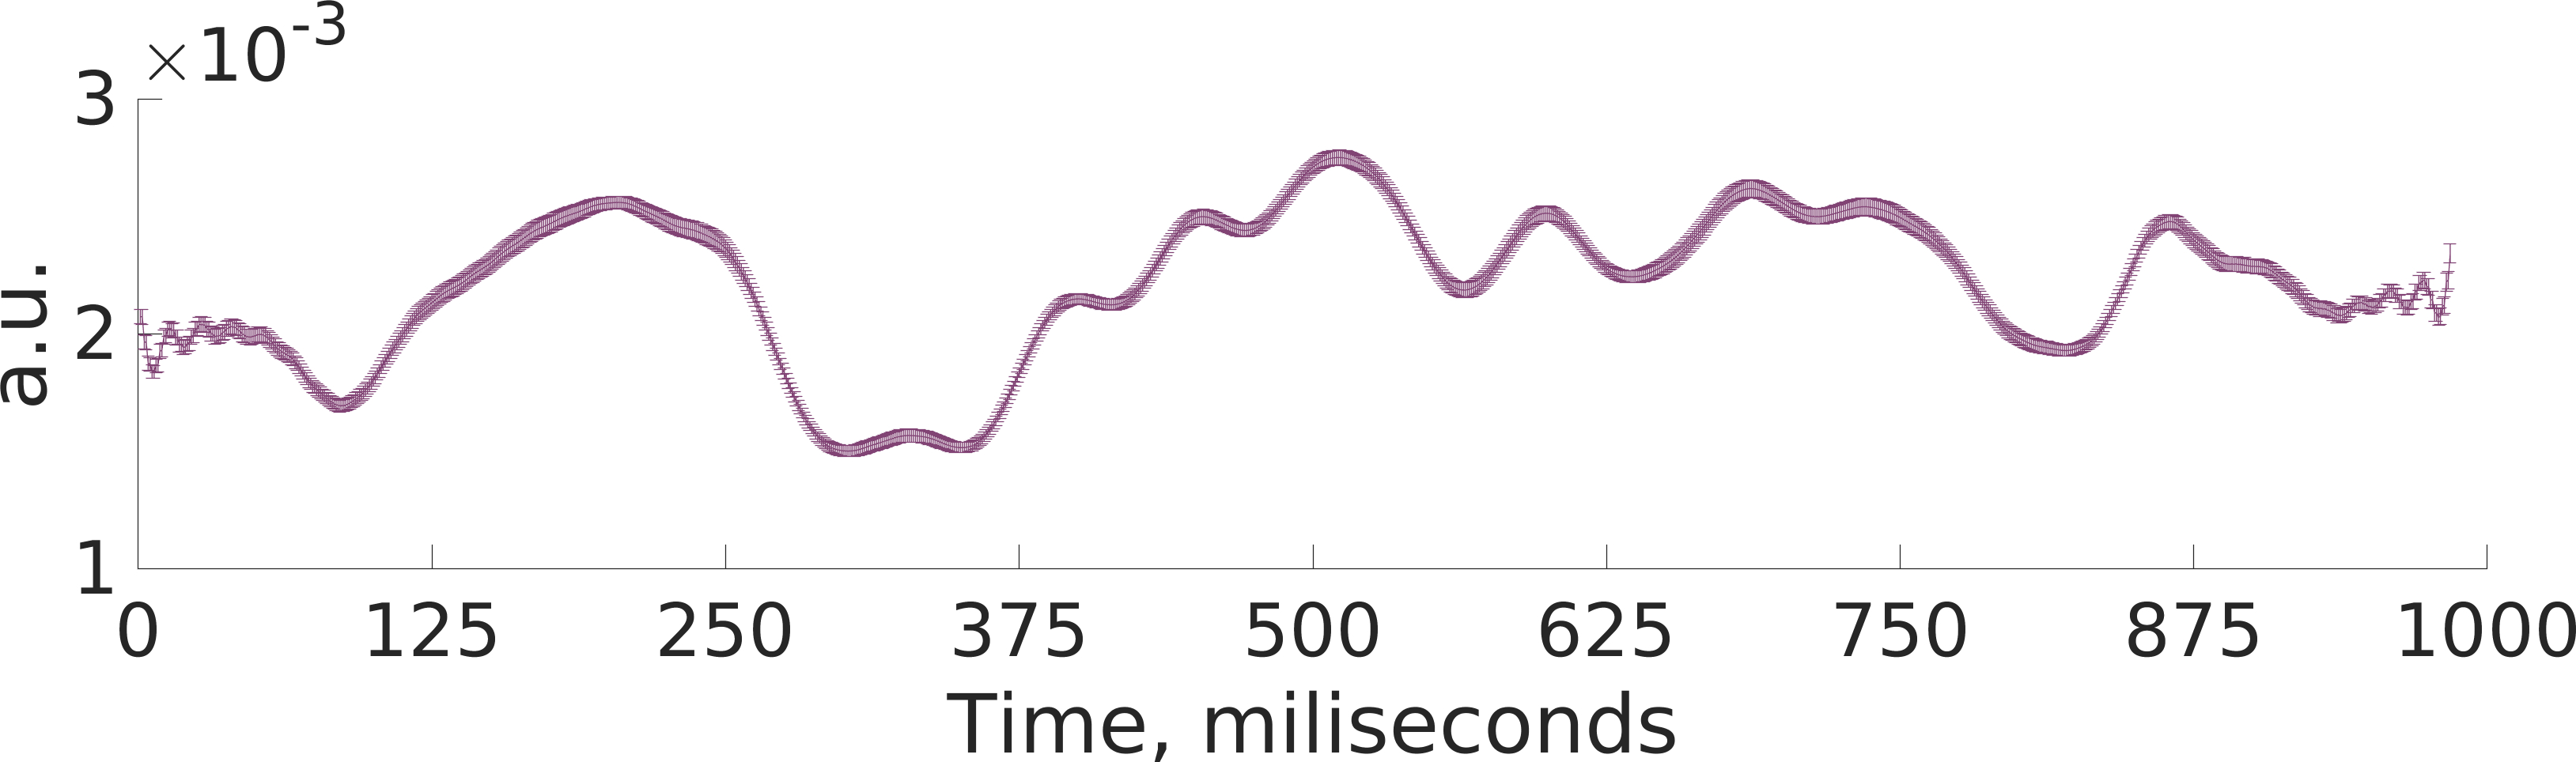
\includegraphics[width=\textwidth]{../images/psiicos_paper/Figure13_b2.jpg}
 \caption{Верх. гамма-диапазон, Re, сеть 1}\label{fig:13b}
 \end{subfigure}

 \begin{subfigure}[b]{0.4\textwidth}
 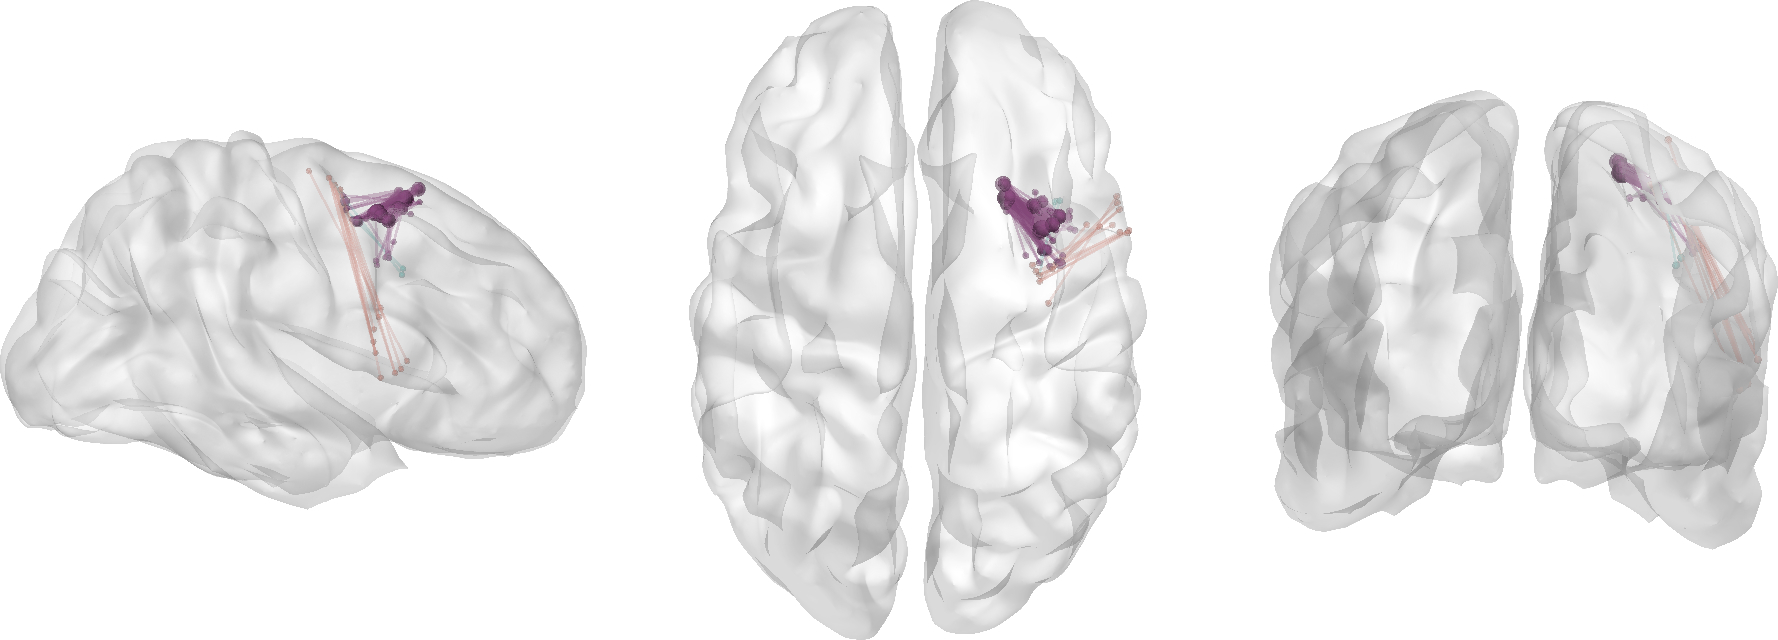
\includegraphics[width=\textwidth]{../images/psiicos_paper/Figure13_c1.jpg}
 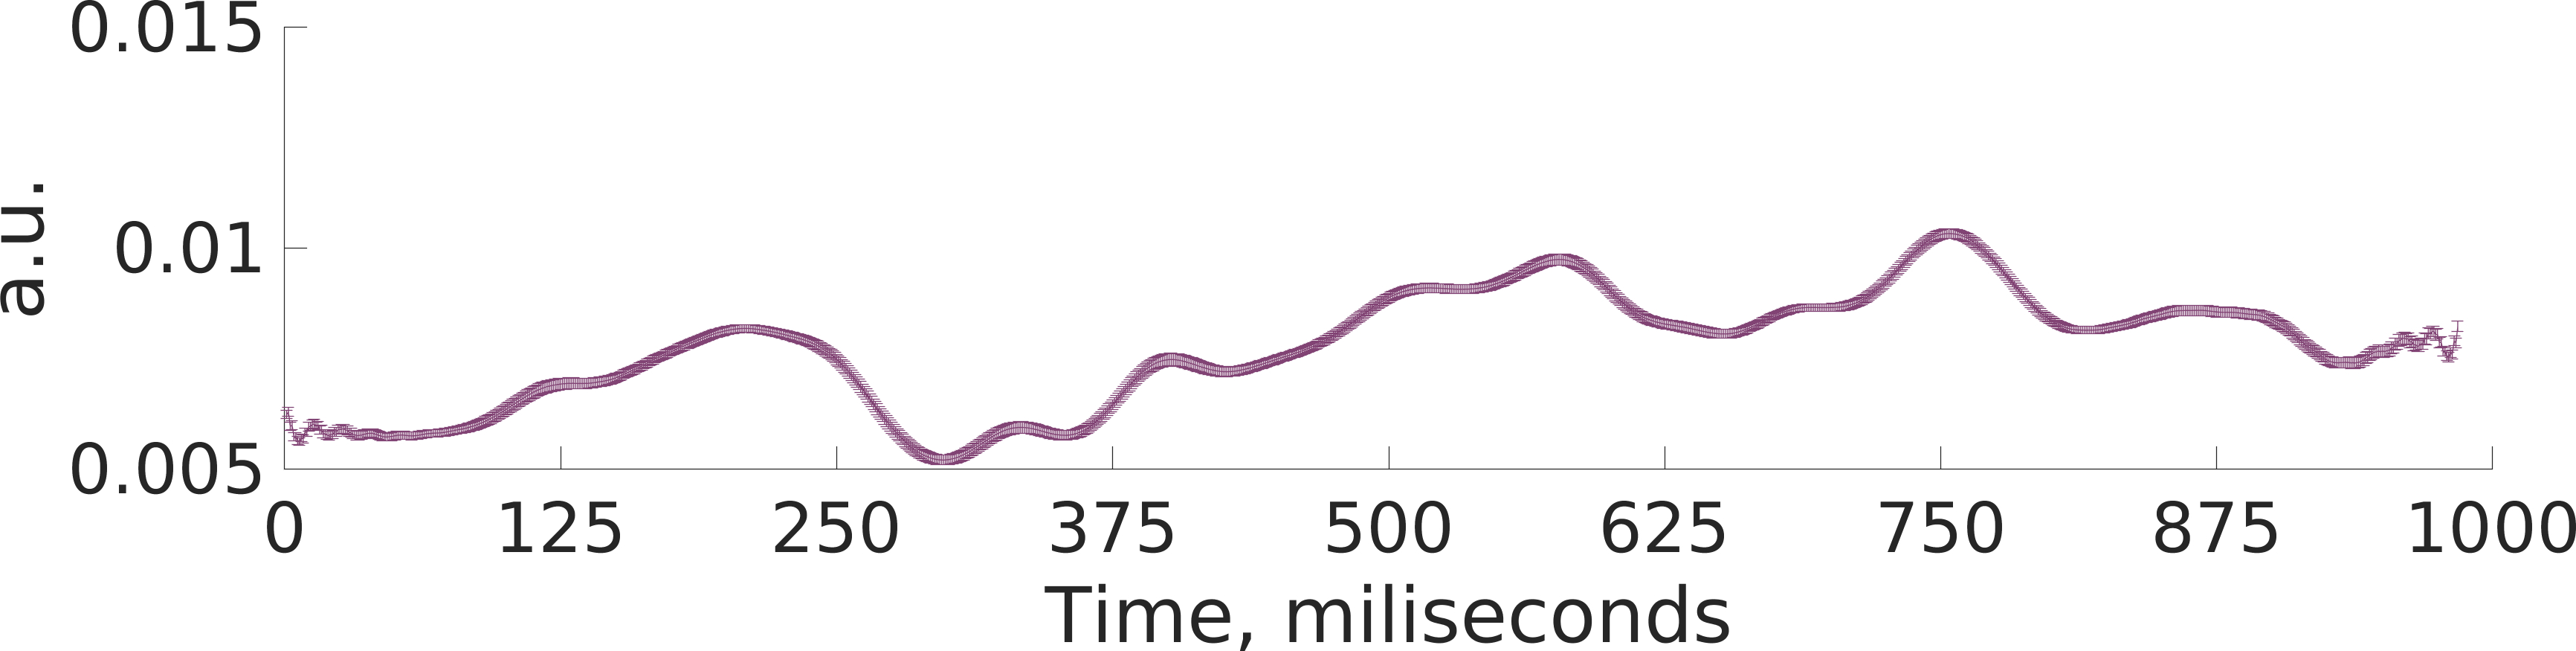
\includegraphics[width=\textwidth]{../images/psiicos_paper/Figure13_c2.jpg}
 \caption{Ниж. гамма-диапазон, Im, сеть 1}\label{fig:13c}
 \end{subfigure}
 \caption{Пространственная структура и временная динамика наиболее воспроизводимых сетей в нижнем (30--60 Гц) и верхнем (65--85 Гц) гамма-диапазонах}\label{fig:13}
\end{figure} % Figure 13

Сети, найденные по мнимой части кросс-спектра, включают связь в альфа-диапазоне
билатеральных сенсорных областей со срединной внутренней поверхностью
коры,~\ref{fig:11b}, а также кросс-латеральные связи между относящимися к руке
зонами сенсорной коры в бета-диапазоне,~\ref{fig:12c}.

Мы также сравнили результаты нашего анализа коннективности с
пространственно-специфичным распределением индуцированной мощности по
коре,~\ref{appendix:real_data_power}. Результаты этого сравнения показывают,
что все обнаруженные сети кроме одной билатеральной сети в бета-диапазоне не
демонстрируют ситуации, когда оба узла сети лежат в областях с высокой
мощностью. В то же время, сенсомоторная область правого полушария, будучи узлом
большинства найденных сетей, совпадает с областью наибольшей активации. Так как
правая мотосенсорная кора играет ключевую роль в исходном
исследовании~\cite{DeLange2008} и так как мы оценивали коннективность не для
одной точки с остальными частями коры, а всех точек со всеми, мы находим эти
результаты обнадеживающими.
